\documentclass[12pt,english,a4paper]{report}

\usepackage{thesis}
\usepackage{geometry}
%\usepackage{times}
\usepackage[T1]{fontenc}
\usepackage{epsfig}
\usepackage{graphicx}
\usepackage{amsmath}
\usepackage{amssymb}
\usepackage{array}
\usepackage{setspace}
\usepackage{etoolbox}
\usepackage{tocbibind}
\usepackage[normalem]{ulem}
\usepackage{lipsum}
\usepackage{gensymb}

% Include other packages here, before hyperref.
\usepackage{subcaption}

% For appendix
\usepackage{csvsimple}
\usepackage{rotating}
\usepackage{lscape}

% If you comment hyperref and then uncomment it, you should delete
% egpaper.aux before re-running latex.  (Or just hit 'q' on the first latex
% run, let it finish, and you should be clear).
\usepackage[pagebackref=true,breaklinks=true,letterpaper=true,colorlinks,bookmarks=false]{hyperref}
\hypersetup{
    linkcolor = {}
}

% for displaying textures
%\newcommand{\figsz}{0.47in}
\newcommand{\figsz}{0.87in}
\newcolumntype{V}{>{\centering\arraybackslash} m{\figsz} }
\newcommand{\showtexframe}[1]{\epsfig{file=#1, width = \figsz}}
\newcommand{\showtexture}[1]{
\vspace{0.1cm} \showtexframe{#10.jpeg} \showtexframe{#11.jpeg} \showtexframe{#12.jpeg} \showtexframe{#13.jpeg} \showtexframe{#14.jpeg} %\showtexframe{#15.jpeg} \showtexframe{#16.jpeg} \showtexframe{#17.jpeg} \showtexframe{#18.jpeg}
}
\newcommand{\showtextureshort}[1]{
\vspace{0.1cm} \showtexframe{#10.jpeg} \showtexframe{#11.jpeg} \showtexframe{#12.jpeg} \showtexframe{#13.jpeg} \showtexframe{#14.jpeg}
}

% teletype text to go to newline if overflow
\newcommand\wtt[1]{%
  \hfil\penalty0\hfilneg\texttt{#1}%
}

% for todo
\usepackage{todo}
\usepackage{xcolor}
\DeclareRobustCommand\todomatthew[1]{\textcolor{red}{\Todo[Matthew]{#1}}}

% for highlighting text
\DeclareRobustCommand\highlight[1]{\textcolor{red}{#1}}

% for showing crossed-out text
\newcommand\edit[2]{\sout{#1}\textcolor{red}{#2}}

% include abstract in table of contents
\patchcmd{\abstract}{\titlepage}{%
  \titlepage
  \phantomsection
  \addcontentsline{toc}{chapter}{\abstractname}}{}{}

% acknowledgements is an abstract (to get the same formatting)
\newenvironment{acknowledgements}{\renewcommand\abstractname{Acknowledgements}\begin{abstract}}{\end{abstract}}

% include appendix in table of contents
\newcommand\myappendix[1]{%
  \appendix
  \chapter*{#1}\label{chap:appendix}
  \markboth{\MakeUppercase{#1}}{}
  \refstepcounter{chapter}
  \addcontentsline{toc}{chapter}{#1}}

% fancy page header
\usepackage{fancyhdr}
\pagestyle{fancy}
\renewcommand\chaptermark[1]{\markboth{\MakeUppercase{Chapter~\thechapter: #1}}{}}
\fancyhf{}
\fancyhead[R]{\bfseries\leftmark}
%\fancyhead[R]{\bfseries\thepage}
\fancyfoot[C]{\thepage}
\renewcommand\headrulewidth{0.4pt}% suppress the header rule

%\setcounter{secnumdepth}{3}
%\setcounter{tocdepth}{3}

\graphicspath{{figures/}}

\begin{document}

\begin{titlepage}
	\thispagestyle{empty}
	\setcounter{page}{1}
	\centering
	{\LARGE Two-Stream Convolutional Networks for Dynamic Texture Synthesis\\}
	\vspace{4cm}
	BY\\
	\vspace{0.5cm}
	MATTHEW TESFALDET\\
	\vspace{2cm}
	A THESIS SUBMITTED TO\\
	THE FACULTY OF GRADUATE STUDIES\\
	IN PARTIAL FULFILLMENT OF THE REQUIREMENTS\\
	FOR THE DEGREE OF\\
	MASTER OF SCIENCE\\
	\vspace{1cm}
	GRADUATE PROGRAM IN COMPUTER SCIENCE\\
	YORK UNIVERSITY\\
	TORONTO, ONTARIO\\
	\vspace{1cm}
	August, 2018\\
	\vspace{1cm}
	\copyright \, Matthew Tesfaldet, 2018
\end{titlepage}

\doublespacing

%-----------Roman pages------------%
\pagenumbering{roman}
\begin{abstract}
\thispagestyle{plain}
\setcounter{page}{1}
This thesis introduces a two-stream model for dynamic texture synthesis.
The model is based on pre-trained convolutional networks (ConvNets)
that target two independent tasks: (i) object recognition, and (ii)
optical flow regression.
Given an input dynamic texture, statistics
of filter responses from the object recognition ConvNet
encapsulate the per-frame appearance of the input texture, while
statistics of filter responses from the optical flow ConvNet model
its dynamics.
To generate a novel texture, a randomly initialized input sequence is optimized
to match the feature statistics from each
stream of an example texture.  
In addition, inspired by recent work on image style transfer and enabled by the
two-stream model, the synthesis approach is applied to combine the
texture appearance from one texture with the dynamics of another 
to generate entirely novel dynamic textures.
Overall, the proposed approach generates novel, high quality samples 
that match both the framewise appearance and temporal evolution
of input texture.
Finally, a quantitative evaluation of the proposed dynamic texture synthesis approach is performed via a large-scale user study.
\end{abstract}
\begin{acknowledgements}
\thispagestyle{plain}
\setcounter{page}{2}
%	This thesis is dedicated to my parents, Bereket Tesfaldet and Simret Tesfaldet. Your caring, loving commitment to my well-being and utmost support have taught me the value.
I acknowledge the financial support of the Canadian Graduate Scholarship (CGS) awarded by the Natural Sciences and Engineering Research Council of Canada (NSERC). This research was undertaken as part of the Vision: Science to Applications program, thanks in part to funding from the Canada First Research Excellence Fund.
\end{acknowledgements}
\setcounter{page}{3}
\onehalfspacing
\tableofcontents
\listoftables
\listoffigures
\doublespacing
%----------------------------------%

\newpage
\pagenumbering{arabic}
\setcounter{page}{1}

\chapter{Introduction \todomatthew{almost finished}}

\section{Motivation}

The natural world is rich in visual texture. While a precise definition of 
texture remains to be found, most research consider it as visual patterns that 
exhibit local spatial variations while maintaining global homogeneity \todomatthew{figure of a texture}. Textures 
can be static or dynamic: static textures exist in two-dimensional (2D) image space 
(\eg, grass and water) while dynamic textures extend the notion across time (\eg, 
fluttering grass and wavy water). As a result, local spatial variations and 
global homogeneity extend across space \emph{and} time. These temporal patterns 
have previously been studied under a variety of names, including turbulent-flow 
motion \cite{heeger1986}, temporal textures \cite{nelson1992}, time-varying 
textures \cite{bar-joseph2001}, dynamic textures \cite{doretto2003}, textured 
motion \cite{wang2003} and spacetime textures \cite{derpanis2012spacetime}.
In this thesis, the term ``dynamic texture'' is adopted. \todomatthew{1 sentence for each reference with a short description of the work and the context. }

Both static and dynamic texture cues play important roles in our perception of 
surfaces. Understanding and characterizing these patterns has long been a problem 
of interest in human perception, computer vision, and computer graphics. In 
computer vision, studying the underlying statistics of textures allows us to gain 
insight as to how these complex structures can be interpreted and how we may be 
able to leverage this knowledge to inform certain vision-related tasks. Examples 
of such tasks include shape from texture \cite{gibson1950perception}, texture 
synthesis \cite{heeger1995pyramid}, and more recently, image style transfer 
\cite{gatys2016image}.

Shape from texture involves recovering the
three-dimensional (3D) shape of an object from a 2D image by using texture as a 
cue. Gibson \cite{gibson1950perception} proposed the \emph{texture gradient} as 
the primary basis of surface perception by humans. He revealed that neighbouring areas on a textured surface are perceived differently only due to differences
in surface orientation and distance from the observer.

Texture synthesis \todomatthew{perhaps include a figure of texture synthesis} is the process of algorithmically constructing a texture that
matches or extends a given source texture by taking advantage of its structural 
content. Heeger and Bergen \cite{heeger1995pyramid} took advantage of the fact 
that two textures are often difficult to discriminate when they produce a similar 
distribution of responses from a bank of linear filters. They used a combination 
of Laplacian and steerable pyramids to deconstruct a given texture and 
synthesized a new texture by matching the distributions of responses from each
pyramid level. Image style transfer \todomatthew{include style transfer figure} is a recent extension of texture synthesis where the goal is to 
synthesize a texture from a source image while constraining the process in order 
to preserve the semantic content of another image. This can be considered as a 
texture transfer problem \todomatthew{cite texture transfer papers}. Gatys \etal \cite{gatys2016image} demonstrated 
impressive results by using a convolutional network (ConvNet) instead of a linear 
bank of filters to model the non-linear spatial statistics of a given texture and semantic content of a given image. The focus of this work is on the synthesis of dynamic texture 
samples based on a single exemplar through the use of ConvNets. \todomatthew{discuss the previous use of purely filter driven characterizations of textures and the current use of CNNs.}

\section{Outline of thesis}

Many common dynamic textures are naturally described by the ensemble of 
appearance and dynamics (\ie, spatial and temporal pattern variation) of their 
constituent elements. In this work, a factored analysis of dynamic 
textures in terms of their appearance and dynamics is proposed.
This factorization is then used to enable dynamic texture synthesis
which, based on example dynamic texture inputs, will generate a novel dynamic
texture instance.
It shall also enable a novel form of style transfer where the 
target appearance and dynamics can be taken from different sources---termed \emph{dynamics style transfer}.
An overview of dynamic texture synthesis and dynamics style transfer
is shown in Fig.\ \ref{fig:teaser}.

\begin{figure}[t]
\begin{center}
	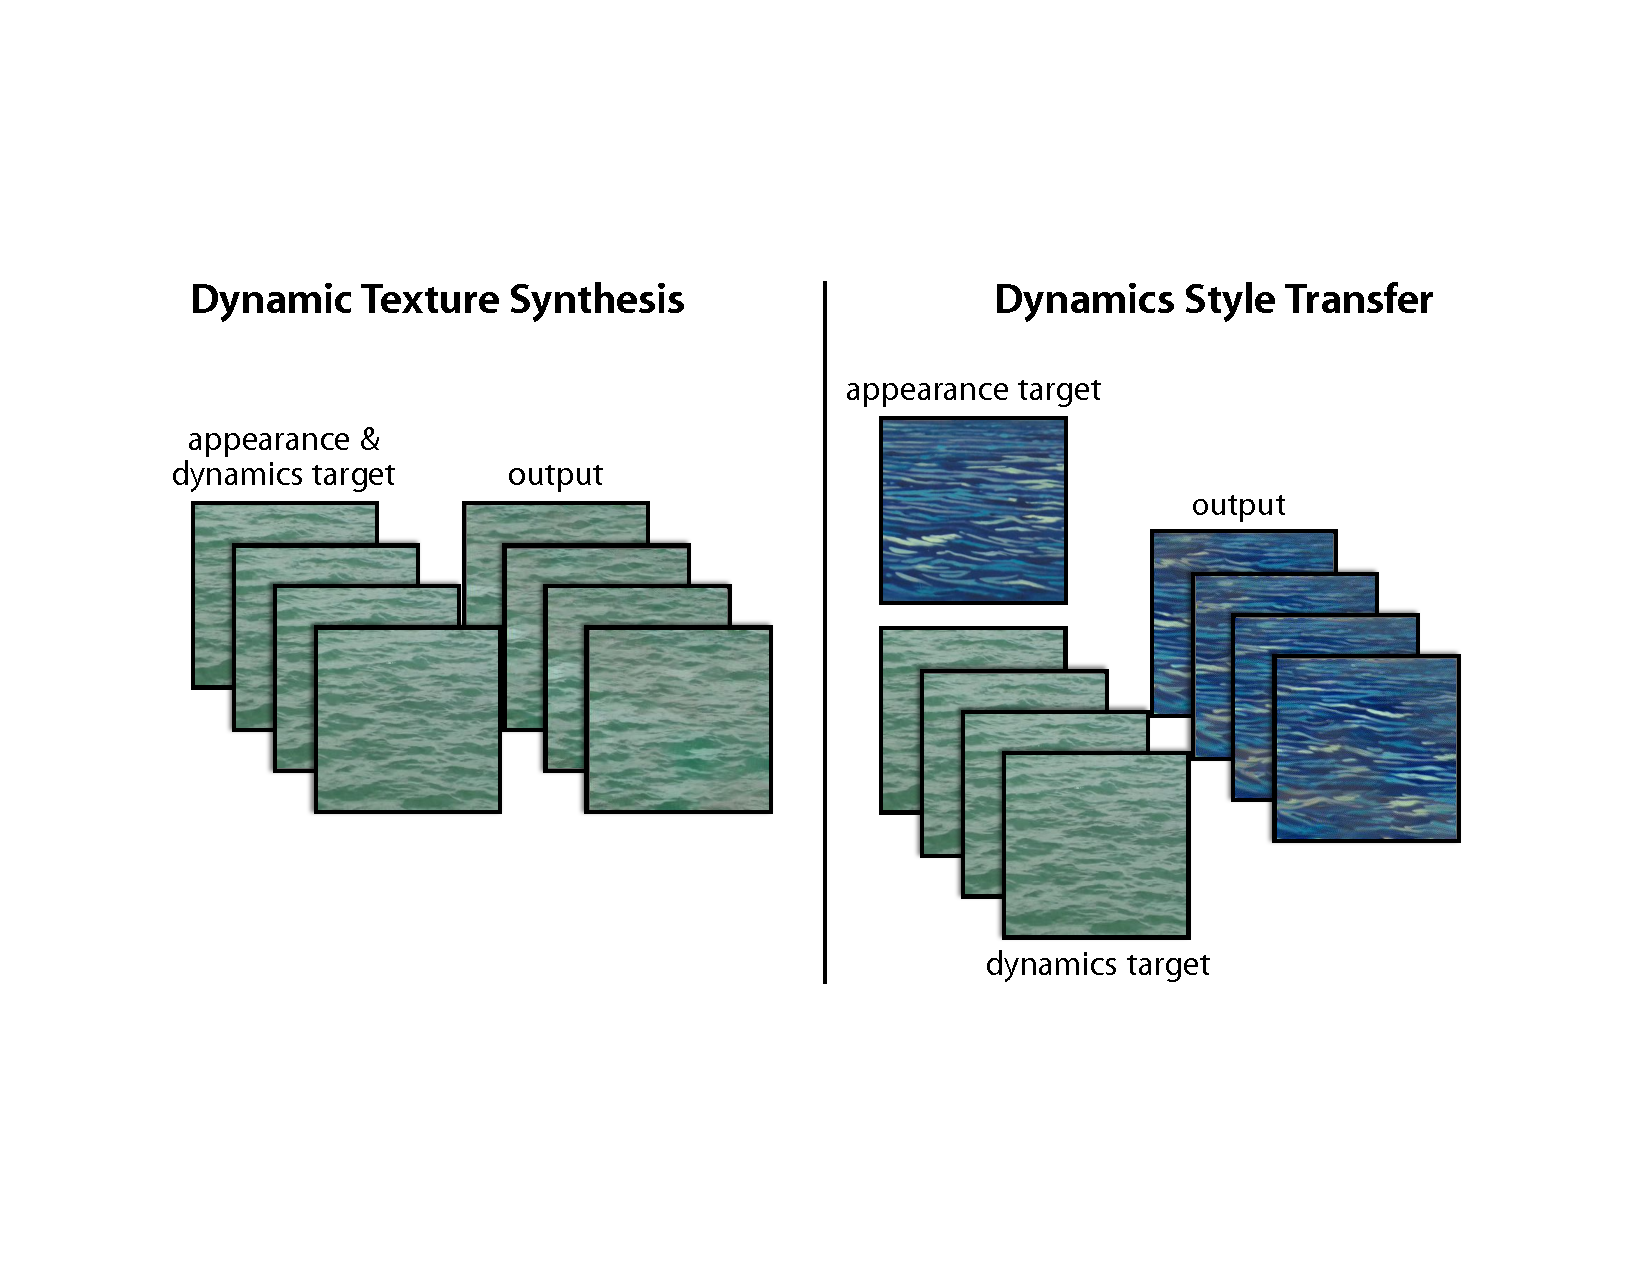
\epsfig{file=teaser.pdf, width = 0.8\textwidth}\\
	\caption[Dynamic texture synthesis.]{Dynamic texture synthesis. (left) Given an input dynamic texture as the target, the two-stream model synthesizes a novel dynamic texture that preserves the target's appearance and dynamics characteristics. (right) The two-stream approach enables synthesis that combines the texture appearance from one target with the dynamics from another, resulting in a composition of the two.}
	\vspace{-0.65cm}
	\label{fig:teaser}
\end{center}
\end{figure}

The proposed model is constructed from two ConvNets: an appearance stream and a dynamics stream,
which have been pre-trained for object recognition
and optical flow prediction, respectively.
Similar to previous work on spatial textures
\cite{gatys2015,heeger1995pyramid,portilla2000parametric}, an input dynamic texture is summarized in terms of a set of
spatiotemporal statistics of filter outputs from each stream.
The appearance stream models the per-frame appearance of
the input texture, while the dynamics stream models its
temporal dynamics.
The synthesis process consists of optimizing a randomly initialized noise pattern such that its spatiotemporal statistics from
each stream match those of the input texture.
The architecture is inspired by insights from human perception and 
neuroscience.
In particular, psychophysical studies \cite{cutting1982} show that
humans are able to perceive the structure of a dynamic texture even
in the absence of appearance cues, suggesting that the two streams
are effectively independent.
Similarly, the two-stream hypothesis \cite{goodale1992} models the 
human visual cortex in terms of two pathways, the ventral stream
(involved with object recognition) and the
dorsal stream (involved with motion processing).

In this thesis, the two-stream analysis of
dynamic textures is applied to texture synthesis.
A range of dynamic textures are considered and it is demonstrated that the 
proposed approach generates novel, high quality samples that match
both the frame-wise appearance and temporal evolution of an input
example.
Further, as stated previously, the factorization of appearance and dynamics enables a 
novel form of style transfer, where the dynamics of one texture are 
combined with the appearance of a different one,
\cf\ \cite{gatys2016image}.
This can even be done using a single image as an appearance
target, which allows static images to be animated.
Finally, the perceived realism of the generated textures is validated
through an extensive user study.

\section{Contributions}

The contributions of this work span both theory and application. First,
theoretical insight into the characterization of dynamic textures is provided by 
building a novel factored representation of both appearance and dynamics. Second, 
for the representation of dynamics, a novel ConvNet is constructed and trained for 
optical flow prediction. Third, through a qualitative evaluation, it is shown that the two-stream representation is 
effective in generating visually compelling, novel instances of a wide range of 
dynamic textures. Fourth, a novel form of style transfer is demonstrated, 
where the dynamics of a dynamic texture can be mixed with the spatial appearance 
of a different (static or dynamic) texture. This is enabled by the proposed factored 
representation. Finally, a quantitative evaluation on the limitations of the method is performed through 
the inclusion of a broad range of textures and an extensive user study. This analysis will show which 
sequences work better than others and why. This may point to future work to 
address limitations of the proposed model. In terms of specific applications, 
there are many in the creative-industry including, but not limited to, computer-
generated imagery, digital painting, and image editing. More broadly, the ability 
to animate static imagery via dynamics style transfer can meaningfully contribute 
to the emerging artistic medium of computer-generated art.

\chapter{Background}\label{chap:background}

This chapter aims to summarize the relevant theory and mathematics of
convolutional networks,
static and dynamic texture synthesis, image style transfer, and representations of dynamics so as to provide sufficient
background information for the following chapters. Research
related to this thesis is covered simultaneously.

\section{Convolutional networks}

A convolutional network (ConvNet) is a feed-forward computational graph of processing nodes, commonly used in analyzing visual imagery. It is a class of artificial neural networks (ANNs), which are computational systems vaguely inspired by the biological neural networks that constitute animal brains. ConvNets perform tasks (\eg, object classification) by processing an input, $\mathbf{X} \in \mathbb{R}^{H_x \times W_x \times C_x}$, in a feed-forward manner via a series of linear and non-linear transformations and producing an output, $\mathbf{Y} \in \mathbb{R}^{H_y \times W_y \times C_y}$, relevant to the task (such as the class of an object). Here $H_\ast \times W_\ast$ represents spatial dimensions and $C_\ast$ represents the  number of channels. Each non-linear transformation acts as a point of demarcation in the network known as a \emph{layer}. ConvNets typically consist of multiple layers, each containing a collection of nodes sometimes called \emph{neurons}. At each spatial-channel location of the input to a layer, a neuron computes local non-linear transformations, \eg, $\sigma(\mathbf{x}) = \max{(0, \phi(\mathbf{x}))}$ (known as the \emph{rectified linear unit} or ReLU \cite{nair2010rectified}). At a single location of the input, $\mathbf{x} \equiv (x, y, z)$, the non-linear transformation performed by this neuron produces an output called an \emph{activation} or \emph{feature}, $\sigma(\mathbf{x}) \in \mathbb{R}$. The set of activations produced by a neuron at every location of the input is known as an \emph{activation map} or \emph{feature map}, $\sigma \in \mathbb{R}^{H_\sigma \times W_\sigma \times C_\sigma}$. At the $l$-th layer of the network and for each location $\mathbf{x}$ of the input map, the input to each neuron is the weighted linear combination of activations from neighbouring neurons at the previous layer, $l-1$:
\begin{equation}
	\begin{aligned}
		\phi^l(\mathbf{x}) &= \left(\mathbf{w}^l * \sigma^{l-1}(\mathbf{x})\right) + b^l\\
		&= \left(\sum_{(i, j, k) \in \Omega} \mathbf{w}^l(i, j, k) \sigma^{l-1}(x - i, y - j, z - k)\right) + b^l\ ,
	\end{aligned}
\end{equation}
where $\mathbf{w}^l$ are the \emph{weights} (or \emph{filter}) of the neuron applied to the input $\sigma^{l-1}(\mathbf{x})$, $\Omega$ is a spatial-channel neighbourhood centered about $\mathbf{x}$, $b^l$ is an offset term known as the \emph{bias}, and $\ast$ represents the \emph{convolution} (or \emph{filtering}) operator. Colloquially, the term ``convolution'' is often used to describe the combined process of convolving over an input and subsequently computing its activation. Convolution is typically done in a sliding window fashion across the entire input. At the base of the ConvNet, inputs are typically images (\eg, RGB image $\mathbf{X} \in \mathbb{R}^{H_x \times W_x \times 3}$), while inputs at intermediate layers are activation maps (\eg, $\sigma \in \mathbb{R}^{H_\sigma \times W_\sigma \times C_\sigma}$). 

ConvNets ``learn'' to perform tasks through an iterative process called \emph{training}. At each iteration, an input is fed through the network to produce an output which is subsequently evaluated against the ``true'' output for the given input. This evaluation is known as the \emph{loss function} and represents the network's performance on the task. Implicitly, it also represents the objective the network must achieve (\eg, minimizing classification error). Starting from the loss, the network adjusts its weights and biases at each layer via the gradient of the loss with respect to the weights and biases at that layer. After a suitable amount of training iterations, this \emph{gradient descent} process will be stopped.

\section{Parametric texture synthesis}

Texture synthesis is the process of algorithmically constructing a texture that
matches or extends a given source texture by taking advantage of its structural 
content. There are two general approaches that have dominated the texture
synthesis literature: non-parametric sampling approaches that
synthesize a texture by sampling pixels of a given source texture
\cite{efros1999,kwatra2003graphcut,schodl2000,wei2000}, and 
statistical parametric models that aim to synthesize a texture by sampling
from a parameterized model of the source texture.
As the proposed approach is an instance of a parametric model, this thesis 
will focus on these parametric approaches.

The statistical characterization of visual textures was introduced
in the seminal work of Julesz \cite{julesz1962}.
He conjectured that particular statistics of pixel intensities
were sufficient to partition textures into metameric (\ie,
perceptually indistinguishable) classes. 
Later work leveraged this notion for static texture synthesis
\cite{heeger1995pyramid,portilla2000parametric}.
In particular, inspired by models of the early stages of visual 
processing, statistics of (handcrafted) multi-scale oriented filter 
responses were used to optimize an initial noise pattern 
to match the filter response statistics of an input texture.

More recently, Gatys \etal \cite{gatys2015} demonstrated
impressive results by replacing the linear filter bank with the VGG-19
\cite{simonyan2014very} ConvNet pre-trained on the ImageNet \cite{russakovsky2015} dataset for the task of object
recognition. This ConvNet, in effect, served as a proxy for the ventral visual
processing stream. 
Textures were modelled in terms of the normalized correlations between activation maps within several layers of the network.

\subsection{Texture synthesis using a convolutional network}
\label{sec:texture_synthesis_using_a_convnet}

Since the two-stream approach to dynamic texture synthesis proposed by this thesis is an extension of the above texture 
synthesis model, it is useful to describe their approach here. Given a target texture as input,
let $\mathbf{A}^{l} \in \mathbb{R}^{N_l\times M_l}$
be its row-vectorized activation maps at the $l$-th layer of a ConvNet (VGG-19 in the case of Gatys \etal \cite{gatys2015}), where $N_l$ and $M_l$ denote the number of
activation maps and the number of spatial locations,
respectively. The normalized correlations between activation maps
within a layer are encapsulated by a Gram matrix,
$\mathbf{G}^l \in \mathbb{R}^{N_l \times N_l}$, whose entries are given by:
\begin{equation}
	G_{ij}^l = \frac{1}{N_l M_l} \sum_{k=1}^{M_l} A_{ik}^l A_{jk}^l\ ,
\end{equation}
where $A_{ik}^l$ denotes the activation of feature $i$ at
location $k$ in layer $l$ on the target texture. Note that the Gram matrix assumes spatial invariance of the activation statistics.
Given a synthesized texture as input, similarly, let its row-vectorized activation maps
be $\hat{\mathbf{A}}^{l} \in \mathbb{R}^{N_l\times M_l}$ and its normalized
activation map correlations be the Gram matrix, $\hat{\mathbf{G}}^l \in \mathbb{R}^{N_l \times N_l}$, whose entries are given by:
\begin{equation}
	\hat{G}_{ij}^l = \frac{1}{N_l M_l} \sum_{k=1}^{M_l} \hat{A}_{ik}^l \hat{A}_{jk}^l\ .
\end{equation}
The final objective is defined as the average of the mean squared error between
the Gram matrices of the target texture and that of the synthesized texture:
\begin{equation}
   \mathcal{L} = \frac{1}{L} \sum_{l} \Vert \mathbf{G}^l - \hat{\mathbf{G}}^l \Vert^2_F\ ,
   \label{eq:tex_loss}
\end{equation}
where $L$ is the number of VGG-19 layers used when computing Gram matrices
and $\Vert \cdot \Vert_F$ is the Frobenius norm. Gram matrices are computed on
layers \emph{conv1\_1}, \emph{pool1}, \emph{pool2}, \emph{pool3}, and \emph{pool4}.

Before synthesizing a texture, an initial forward pass through VGG-19 is
performed with the target texture as input. The target texture's Gram matrices
across various layers in the network are computed and saved as objectives for
the synthesis process. Then the synthesized texture is initialized with IID
Gaussian noise. The final
objective (Eq.\ \ref{eq:tex_loss}) is minimized with respect to the synthesized texture. With each
iteration of the optimization process, the synthesized texture is updated to appear increasingly
perceptually similar to the target texture. An overview of this process is presented in Fig.\ \ref{fig:vgg_texture_synthesis}.
\clearpage
\begin{figure}[t]
\begin{center}
	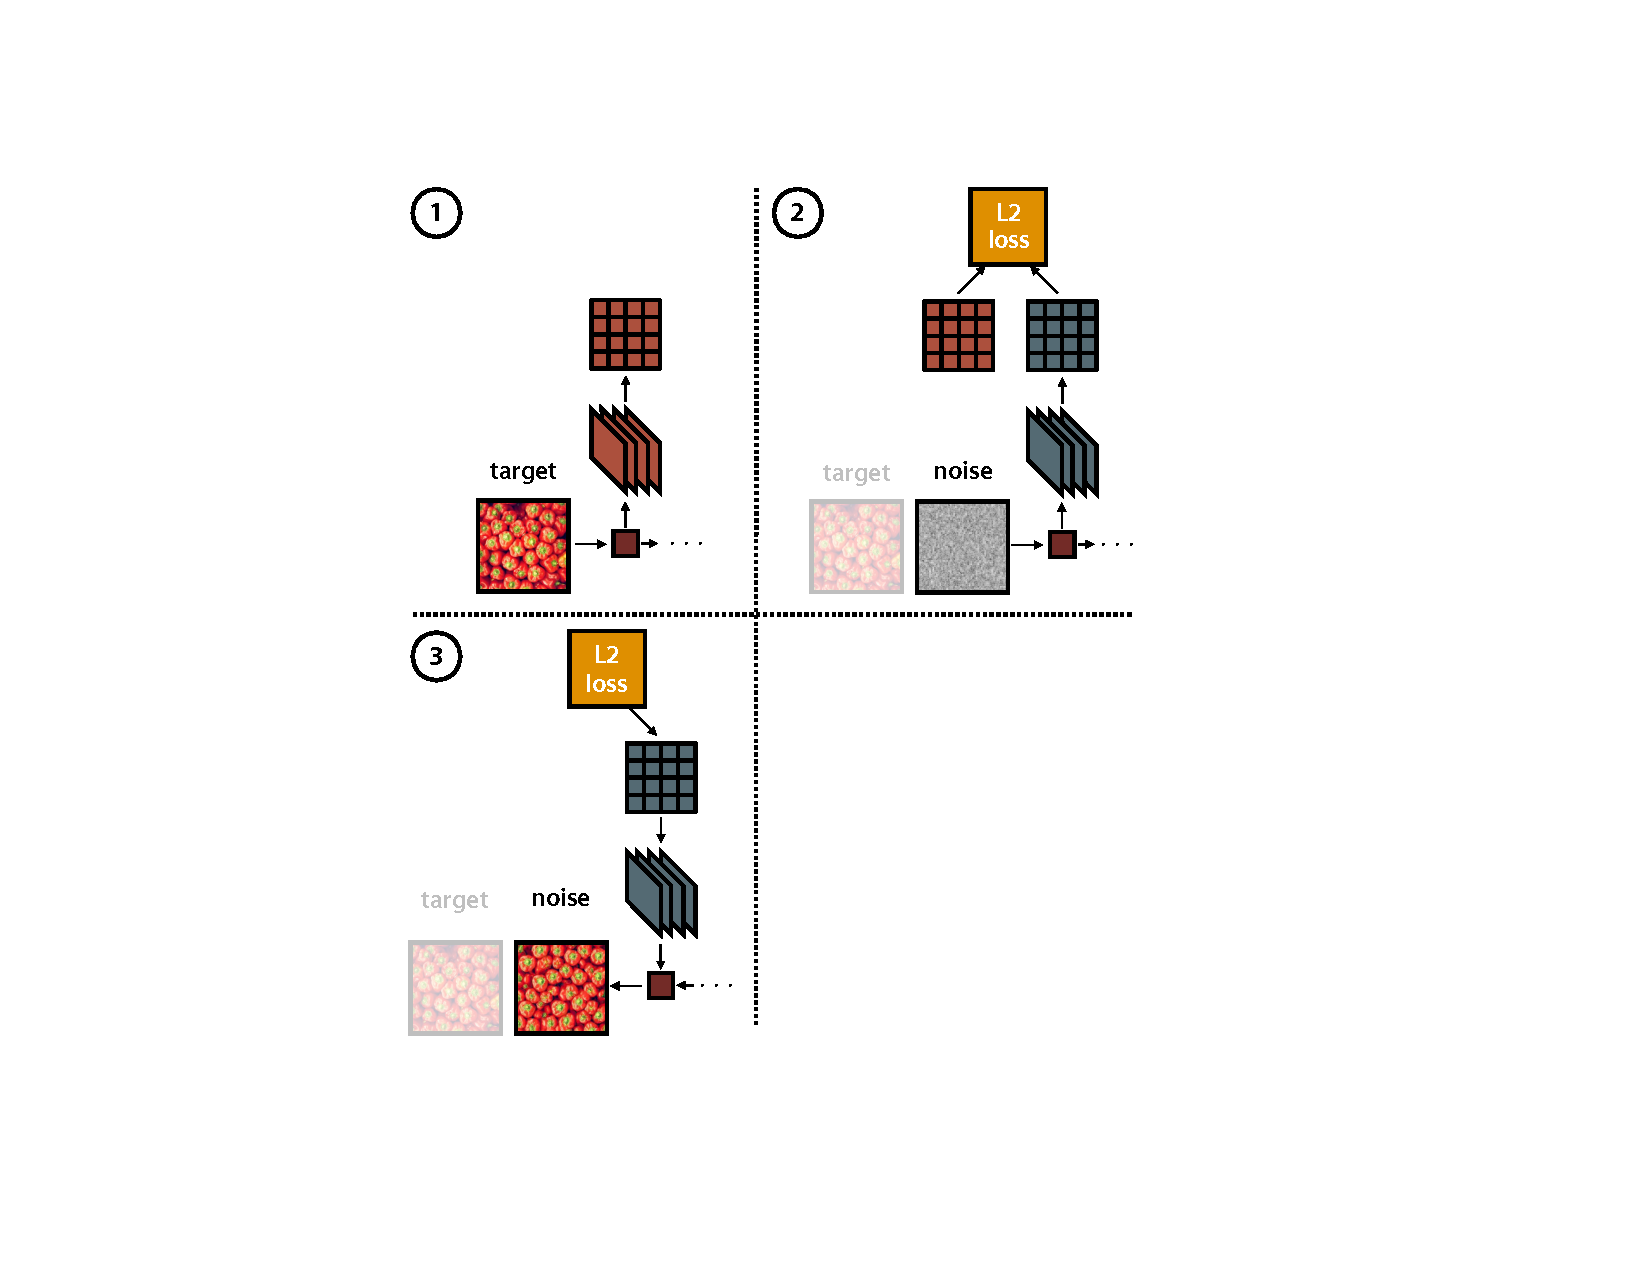
\epsfig{file=vgg_texture_synthesis.pdf, width = \textwidth}\\
	\caption[Static texture synthesis with a convolutional network]{Gatys \etal's \cite{gatys2015} approach to static texture synthesis with the VGG-19 \cite{simonyan2014very} convolutional network. Only the first layer of VGG-19 is shown. (1) An initial forward pass is
performed with the target texture. Its Gram matrices
across various layers are computed and saved. (2) The total L2 loss between the synthesized texture's Gram matrices and the target's is computed. (3) The loss is optimized with respect to the synthesized texture (with the weights of VGG-19 fixed), updating it to appear perceptually similar to the target.}
	\vspace{-0.65cm}
	\label{fig:vgg_texture_synthesis}
\end{center}
\end{figure}
\clearpage

\subsection{The Gram matrix as a texture metric}

Before explaining the Gram matrix as a suitable texture metric, it is necessary to first understand the mathematics behind it. Simply, the Gram matrix of a set of vectors $v_1, \dots , v_n$ in an inner product space is the Hermitian matrix of inner products, whose entries are given by $G_{ij} = \langle v_i, v_j \rangle$ (a Hermitian matrix is a complex square matrix, $A$, that is equal to its own conjugate transpose, \ie, $A = \overline{A^\top}$). Since the inner product space of activation maps is over the real number field, the Gram matrix is also a symmetric matrix. Essentially, the Gram matrix is a covariance matrix describing which of its input vectors are correlated with each other. In the case of Gatys \etal's texture synthesis with a ConvNet, the set of vectors used to compute the Gram matrix are row-vectorized activation maps (Fig.\ \ref{fig:gram_matrix}).
\begin{figure}[t]
\begin{center}
	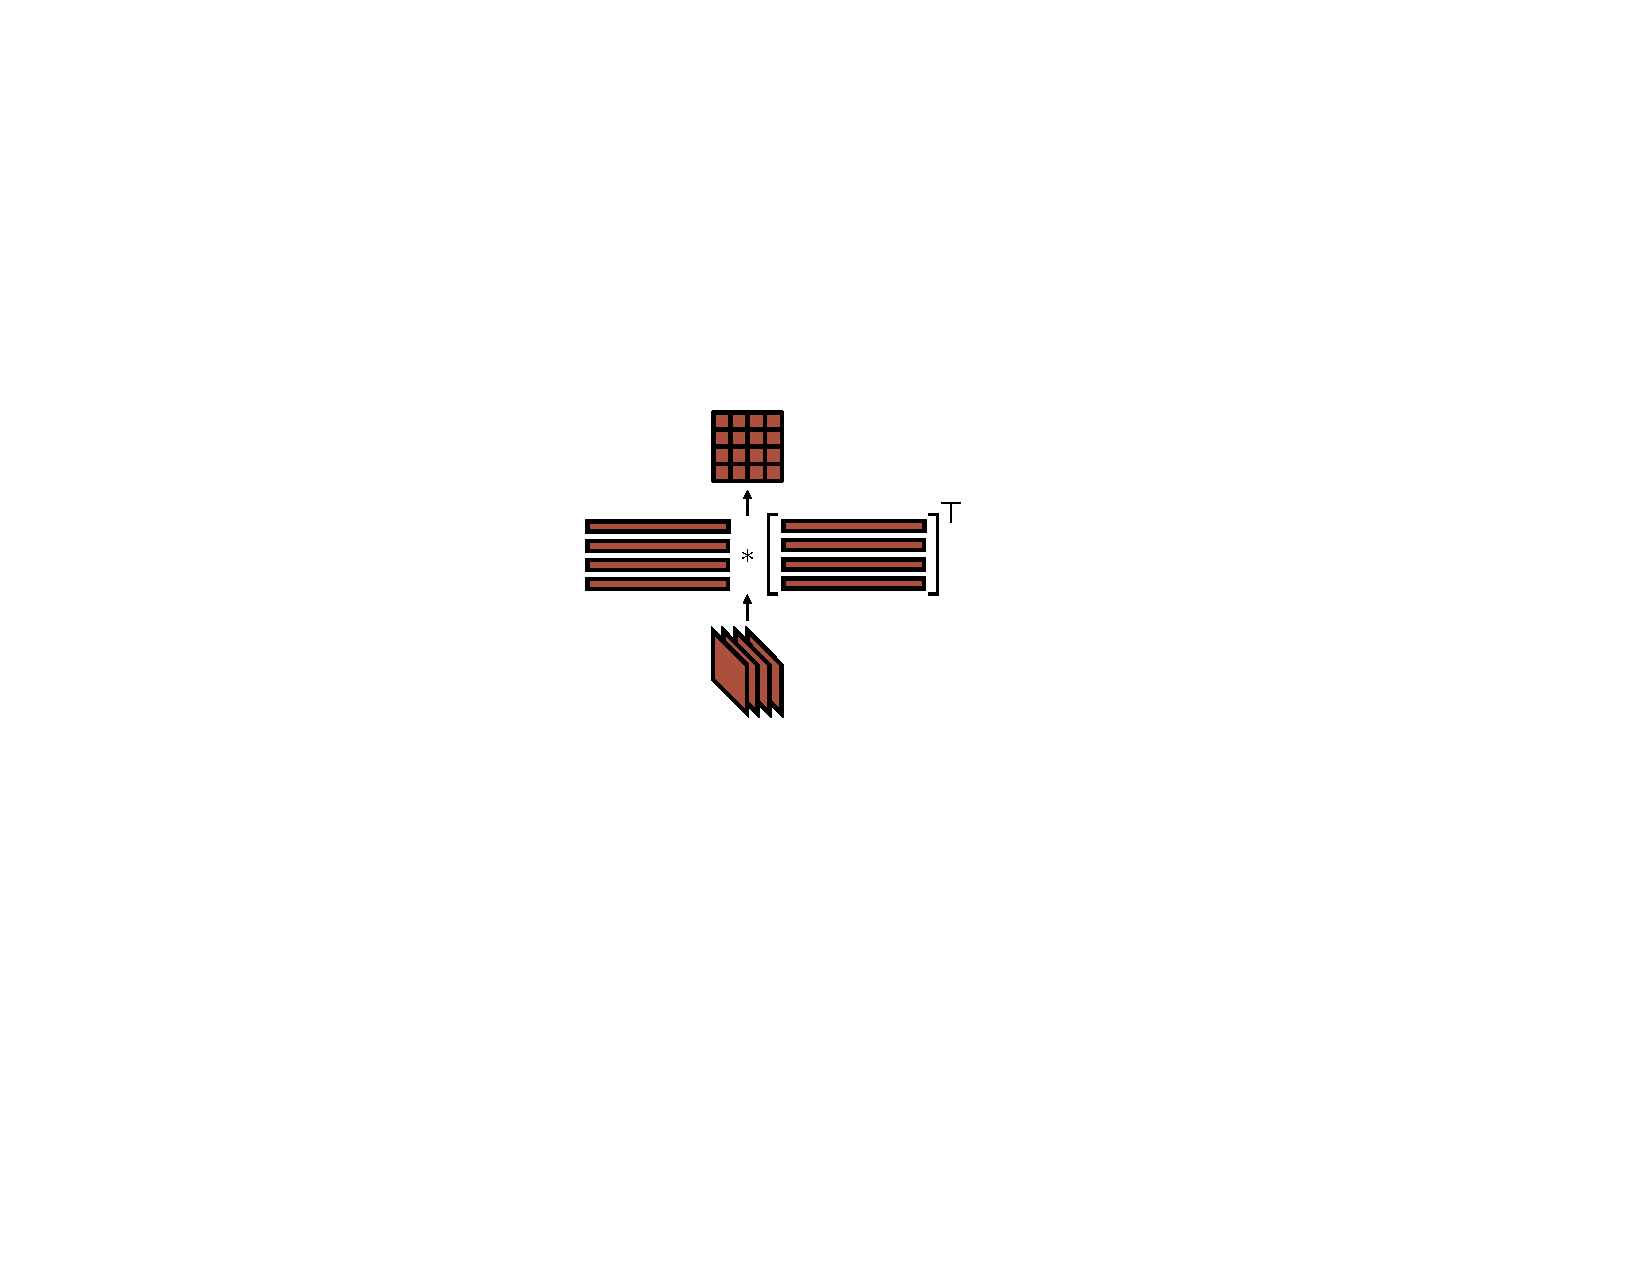
\epsfig{file=gram_matrix.pdf, width = 0.6 \textwidth}\\
	\caption[Computing the Gram matrix from activation maps]{Computing the Gram matrix from the activation maps of a layer. Activation maps are first reshaped to row vectors, then the Gram matrix is realized by computing a matrix multiplication between the row-vectorized activation maps and their transpose.}
	\vspace{-0.65cm}
	\label{fig:gram_matrix}
\end{center}
\end{figure}

In texture synthesis, the Gram matrix measures the amount that co-located features tend to activate together. By computing Gram matrices across several layers, a stationary, multi-scale representation of the input image in terms of its texture information is achieved.

\subsection{Image style transfer}

In subsequent work, Gatys \etal's texture model was used in image style
transfer \cite{gatys2016image}, where the style of one image was
combined with the image content of another to produce a new image.
This was achieved by appending an additional term to Eq.\ \ref{eq:tex_loss}
that enforced the synthesized texture to match the semantic content of the given content image. Specifically,
\begin{equation}
   \mathcal{L} = \frac{1}{L_{style}} \sum_{l} \Vert \mathbf{G}^l - \hat{\mathbf{G}}^l \Vert^2_F\ + \frac{1}{L_{content}} \sum_{l} \Vert \mathbf{A}^l - \hat{\mathbf{A}}^l \Vert^2_F\ ,
   \label{eq:styletransfer_loss}
\end{equation}
where $L_{style}$ and $L_{content}$ are the number of VGG-19 layers used when computing Gram matrices and activation maps, respectively. Gram matrices are computed on the same layers as before, and activation maps are computed on layer \emph{conv4\_2}.

To briefly review, the Gram matrix of activation maps conveys a notion of texture, or ``style'', describing which features tend to activate together. Although the style of the style image is preserved, the global arrangement of its features are not. By including the objective of matching the features of the content image, however, the global arrangement of semantic image content from the content image is preserved. This results in a synthesized image that contains the content of the content image and the style of the style image.

\section{Dynamic texture synthesis}

Dynamic textures extend from static textures with an additional temporal dimension. The stationarity of spatial statistics of static textures also applies to the temporal domain of dynamic textures.

Unlike static texture synthesis, dynamic texture synthesis has not been as deeply explored. Somewhat related to dynamic texture synthesis, Ruder \etal \cite{ruder2016} extended the image style transfer model to video by using
optical flow to enforce temporal consistency of the
resulting imagery. Although their model produced a video output, their core approach focused on an analysis of static texture on a per-frame basis. This is not to be confused with dynamic texture synthesis, which requires an analysis of \emph{dynamic} textures across space \emph{and time}.

Variants of linear autoregressive models have been studied
\cite{szummer1996,doretto2003} that jointly model the appearance and
dynamics of spatiotemporal patterns.
More recent work has considered ConvNets as a basis for modelling 
dynamic textures.
Xie \etal \cite{xie2017synthesizing} proposed a spatiotemporal
generative model where each dynamic texture is modelled as a random
field defined by multiscale, spatiotemporal ConvNet filter responses
and dynamic textures are realized by sampling the model.
Unlike the approach proposed by this thesis, which assumes pre-trained fixed networks,
this approach requires the ConvNet weights to be trained using the
input texture prior to synthesis.

A recent preprint from Funke \etal \cite{funke2017} described preliminary 
results extending the framework of Gatys \etal \cite{gatys2015} 
to model and  synthesize dynamic textures by computing a Gram 
matrix of filter activations over a small spatiotemporal window.
In contrast, the proposed two-stream filtering architecture is more 
expressive as the dynamics stream is specifically tuned to 
spatiotemporal dynamics.
Moreover, the factorization
in terms of appearance and dynamics enables a novel form of
style transfer, where the dynamics of one pattern are 
transferred to the appearance of another to generate an
entirely new dynamic texture.
This work is the first to demonstrate this form of style transfer.


\section{Representations of dynamics}

Numerous representations of dynamics in temporal imagery have been explored, each with their own limitations and level of abstraction. Adapted from Derpanis' dissertation on the role of representation in the analysis of visual spacetime \cite{derpanis2010role}, Fig.\ \ref{fig:dynamics_representations} illustrates an organization of several extant representations of temporal imagery dynamics.
\begin{figure}[t]
\begin{center}
	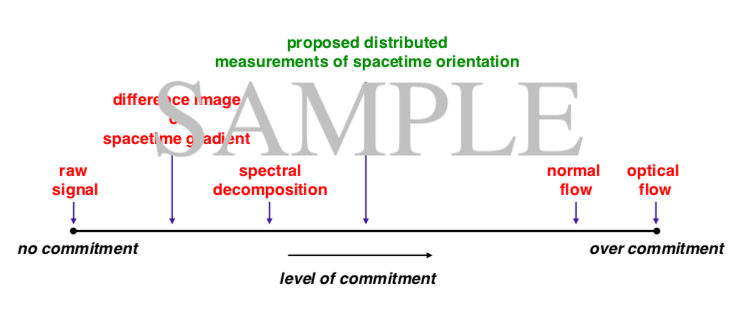
\epsfig{file=dynamics_representations.png, width = \textwidth}\\
	\caption[Dynamics representation spectrum]{Dynamics representation spectrum (adapted from Derpanis \cite{derpanis2010role}). Common abstractions of dynamics of temporal imagery and their respective level of commitment to an underlying model.}
	\vspace{-0.65cm}
	\label{fig:dynamics_representations}
\end{center}
\end{figure}
At one extreme, no commitment to an abstraction is made, the raw signal is used directly (\eg, pointwise intensity and colour). This representation fails to leverage the rich underlying structure in the data. The remaining representations are discussed below.

\subsection{Optical flow}

At the other extreme of Fig.\ \ref{fig:dynamics_representations}, a two-dimensional (2D) vector field is used to represent the dynamics of the input temporal imagery. This vector field is known as \emph{optical flow}. It is used to represent the apparent motion of image pixels between two consecutive frames that is caused by the movement of objects or the camera. Each vector in the 2D vector field is a displacement vector consisting of a horizontal and vertical component, describing the movement of pixels from the first frame to the second. Fig.\ \ref{fig:optical_flow} provides a useful visualization of optical flow.
\begin{figure}[t]
\begin{center}
	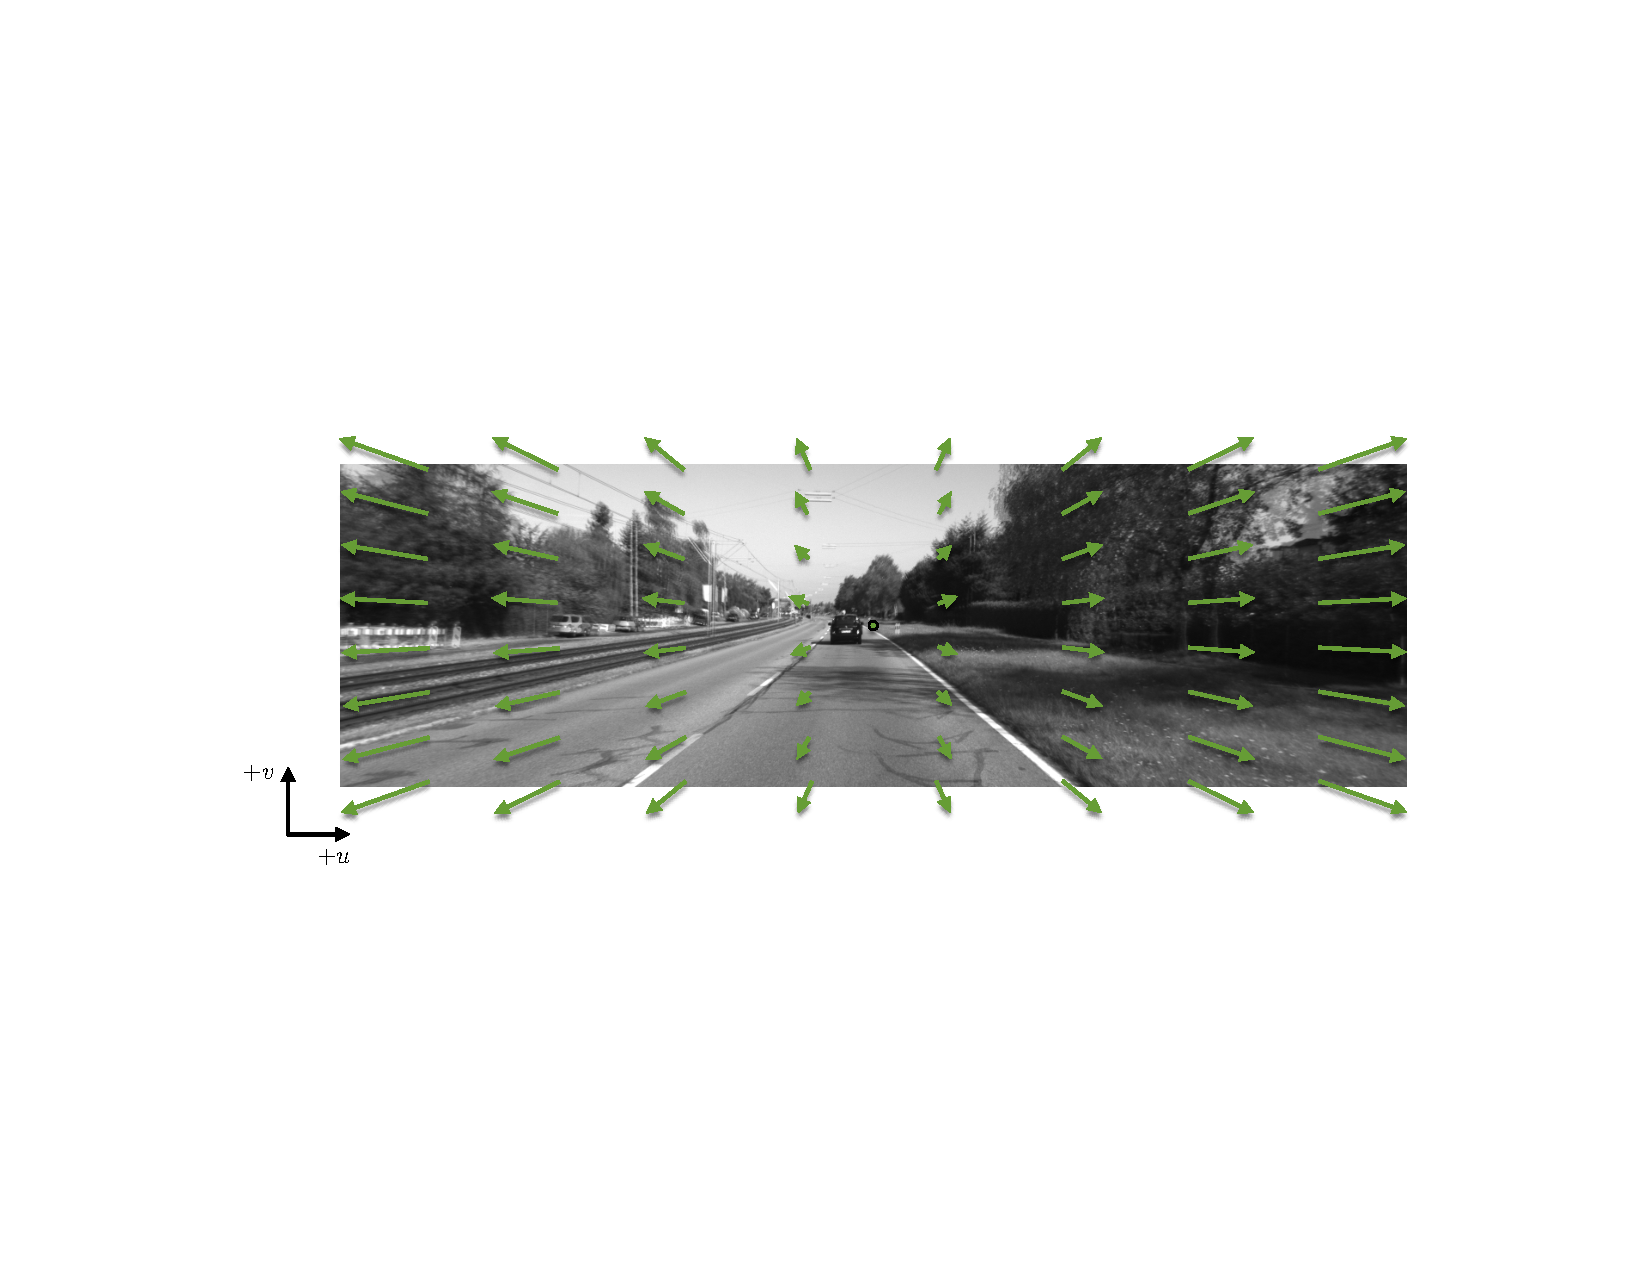
\epsfig{file=optical_flow.pdf, width = \textwidth}\\
	\caption[Optical flow visualization]{Optical flow visualization. Optical flow is a 2D displacement vector field used to represent the apparent motion of image pixels between two consecutive frames, caused by the movement of objects or the camera. Pictured are two, super-imposed, consecutive frames taken from the KITTI dataset \cite{geiger2013vision}. The corresponding optical flow is visualized as an array of green arrows. Note that this is just a sample of the motions that optical flow can characterize.}
	\vspace{-0.65cm}
	\label{fig:optical_flow}
\end{center}
\end{figure}
The recovery of optical flow from temporal imagery has long been studied in computer vision. Traditionally, it has been addressed by handcrafted approaches \eg, \cite{horn1981,lucas1981,revaud2015epicflow}. Recently, ConvNet approaches have been demonstrated as viable alternatives \cite{dosovitskiy2015,ilg2017,ranjan2017,yu2016}.

A limitation of optical flow is its reliance on a single coherent movement for each pixel and its underlying assumption on brightness constancy, which is difficult to justify for the dynamics one may encounter in the real world. Examples of dynamics optical flow would fail to capture include flickering, semi-transparent motion, and stochastic dynamics. These are dynamics typically existent in dynamic textures. Therefore, optical flow is not an optimal measure for representing the dynamics existent in dynamic textures.

\subsection{Marginalized spacetime oriented energies}
\label{sec:msoe}

At the midpoint between the two extremes lies the representation of dynamics that aims to capture a distribution of measurements of spacetime orientations in the input temporal imagery. Unlike flow-based analyses which focus on the apparent motion (\ie translation) present in the data, measurements of spacetime orientations take a geometric and generalized approach in capturing \emph{spacetime structures}: oriented structures in visual spacetime that manifest themselves as motion or non-motion (\eg flickering, stochastic dynamics, etc.). This is visualized in Fig.\ \ref{fig:spacetime_structures} alongside their frequency-space counterparts. 
\clearpage
\begin{figure}[t]
\begin{center}
	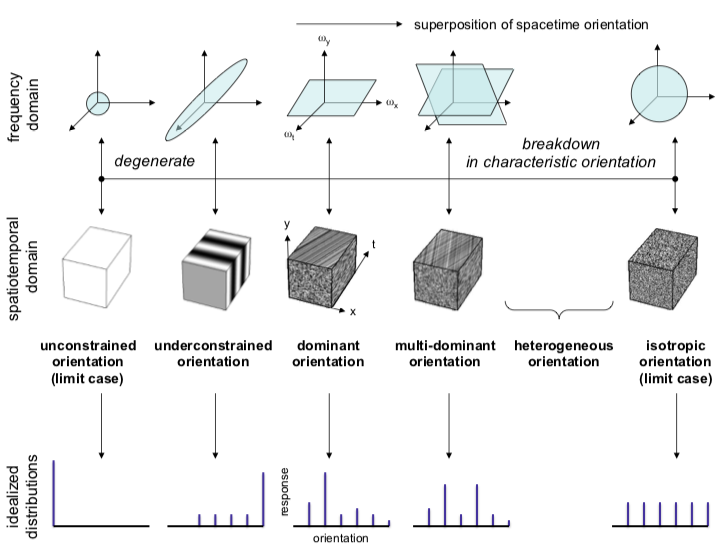
\epsfig{file=spacetime_structures.png, width = \textwidth}\\
	\caption[Spacetime texture spectrum]{Dynamic texture spectrum (adapted from Derpanis \cite{derpanis2012spacetime}). The top and middle rows depict prototypical dynamic textures in the frequency and spatiotemporal domains, respectively. From left-to-right, an increasing amount of spacetime structures are superimposed in a texture. The bottom row depicts a seven bin histogram of the relative spacetime-oriented structure (or lack thereof) present in each dynamic texture. The first histogram bin captures lack of structure. The remaining histogram bins from left-to-right correspond to spacetime orientations selective for static, rightward motion, upward motion, leftward motion, downward motion and flicker structure.}
	\vspace{-0.65cm}
	\label{fig:spacetime_structures}
\end{center}
\end{figure}
\clearpage

Specifically, this thesis adopts the Marginalized Spacetime Oriented Energy (MSOE) approach of Derpanis \etal \cite{derpanis2010role,derpanis2012spacetime} in representing the observed dynamics of a dynamic texture. This representation was successfully used for the task of dynamic texture recognition \cite{derpanis2012spacetime}; here it is used for the task of dynamic texture synthesis.

Most closely related to this approach are energy models of visual
motion \cite{adelson1985spatiotemporal,heeger1988,simoncelli1998,nishimoto2011,derpanis2012spacetime,konda2014}
that have been motivated and studied in a variety of contexts,
including computer vision, visual neuroscience, and visual
psychology.
Given an input image sequence, these models consist of an
alternating sequence of linear and non-linear operations that yield
a distributed representation (\ie,  implicitly coded) of pixelwise
optical flow.
Here, an MSOE model motivates the
representation of observed dynamics which will then be encoded
as a ConvNet. Significantly, a completely analytically-defined
oriented energy ConvNet model provides the current state-of-the-art
for the related task of dynamic texture recognition \cite{hadji2017}.

In motion energy models, the velocity of image content (\ie, motion)
is interpreted as a 3D orientation in the $x$-$y$-$t$
spatiotemporal domain
\cite{adelson1985spatiotemporal,fahle1981,heeger1988,simoncelli1998,watson1983}, previously defined as a spacetime structure.
In the frequency domain, the signal energy of a translating
pattern can be shown to lie on a plane through the origin
where the slant of the plane is defined by the velocity of
the pattern (Fig.\ \ref{fig:spacetime_structures}).
Thus, motion energy models attempt to identify this 
orientation-plane (and hence the pattern's velocity) via
a set of image filtering operations.
More generally,
the constituent
spacetime orientations for a spectrum of common
visual patterns can serve as a basis for describing the temporal
variation of an image sequence \cite{derpanis2012spacetime}.
This observation suggests that motion energy models may form an
ideal basis for the dynamics stream of the proposed dynamic texture synthesis ConvNet. As stated previously, the spacetime-oriented energy model (MSOE) proposed by Derpanis \etal \cite{derpanis2010role,derpanis2012spacetime} is used to motivate the network architecture. The MSOE model is reviewed here.

Given input temporal imagery, $\mathbf{I} \in \mathbb{R}^{T \times H \times W}$ (time $\times$ height $\times$ width), a bank of oriented 3D
filters, \eg, Gaussian third derivative filters $G_3 \in \mathbb{R}^{T \times H \times W}$, which are sensitive to a range of
spatiotemporal orientations, are each applied:
\begin{equation}
	E_{\hat{\theta}} = G_{3_{\hat{\theta}}} \ast \mathbf{I}\ ,
\end{equation}
where $\ast$ denotes convolution, and $G_{3_{\hat{\theta}}}$ is a Gaussian third derivative filter oriented in the direction of the 3D unit vector $\hat{\theta}$ which lies along the filter's symmetry axis. Each of these filtering operations results in a spacetime volume of filter responses, $E_{\hat{\theta}}$.
These filter responses are then rectified (squared) and
pooled over local spacetime regions to make the responses robust
to the phase of the input signal, \ie, robust to the
alignment of the filter with the underlying image
structure:
\begin{equation}
	\bar{E}_{\hat{\theta}} = \sum_{(x, y, t) \in \Omega}{{E_{\hat{\theta}}(x, y, t)}^2}\ .
\end{equation}
At this point, each oriented energy measurement is confounded with spatial orientation. Consequently, in cases where the 
spatial image structure varies wildly about an otherwise coherent dynamic
region, the responses of the bank of oriented filters will reflect this
behaviour and thereby become dependent on spatial appearance; whereas, a description consisting purely 
of pattern dynamics is sought.
To remove this difficulty, the spatial orientation component of each filter is discounted via ``marginalization''. Specifically, filter responses consistent with the same temporal orientation (not necessarily the same spatial orientation), $\hat{\theta}_i$, are summed:
\begin{equation}
	E_{\hat{\mathbf{n}}} = \sum_{i = 1}^{N}{E_{\hat{\theta}_i}}\ ,
	\label{eq:oriented_filter_2.8}
\end{equation}
where $\hat{\mathbf{n}}$ denotes the unit normal of the plane in frequency-space that the spacetime structures captured by these filters lie upon (implicitly describing a single temporal orientation), and $N$ denotes the number of these filters.
For example, in the case where a spacetime structure is defined by the image velocity $(u, v)^\top$ (\ie, optical flow), the unit normal is given by $\hat{\mathbf{n}}=(u, v, 1)^\top / ||(u, v, 1)^\top||$.
These responses provide a pixelwise distributed measure
of which spacetime structures (discounting spatial information) are
present in the input.
However, these responses are confounded by local image
contrast that makes 
it difficult to determine
whether a high response is indicative of the presence of
a spacetime structure or simply due to high image
contrast.
To address this ambiguity, an $\textrm{L}_1$
normalization is applied across oriented filter responses which
results in a representation that is robust to local
appearance variations but highly selective to 
spacetime orientation:
\begin{equation}
	\hat{E}_{\hat{\mathbf{n}}_i} = \frac{E_{\hat{\mathbf{n}}_i}}{\sum_{j = 1}^{M}{E_{\hat{\mathbf{n}}_j}} + \epsilon} \ ,
\end{equation}
where $\hat{E}_{\hat{\mathbf{n}}_i}$ denotes an oriented filter response from Eq.\ \ref{eq:oriented_filter_2.8} corresponding to a plane in frequency-space with unit normal $\hat{\mathbf{n}}_i$.

\chapter{Technical approach \todomatthew{unfinished}}

The proposed two-stream approach consists of an appearance
stream, representing the static (texture) appearance of each frame,
and a dynamics stream, representing temporal 
variations between frames.
Each stream consists of a ConvNet whose activation 
statistics are used to characterize the dynamic texture.
Synthesizing a dynamic texture is formulated as an optimization 
problem with the objective of matching the activation 
statistics.
The dynamic texture synthesis approach is summarized in Fig.\ \ref{fig:architecture}
and the individual pieces are described in turn in the
following sections.

\begin{figure}[t]
\begin{center}
    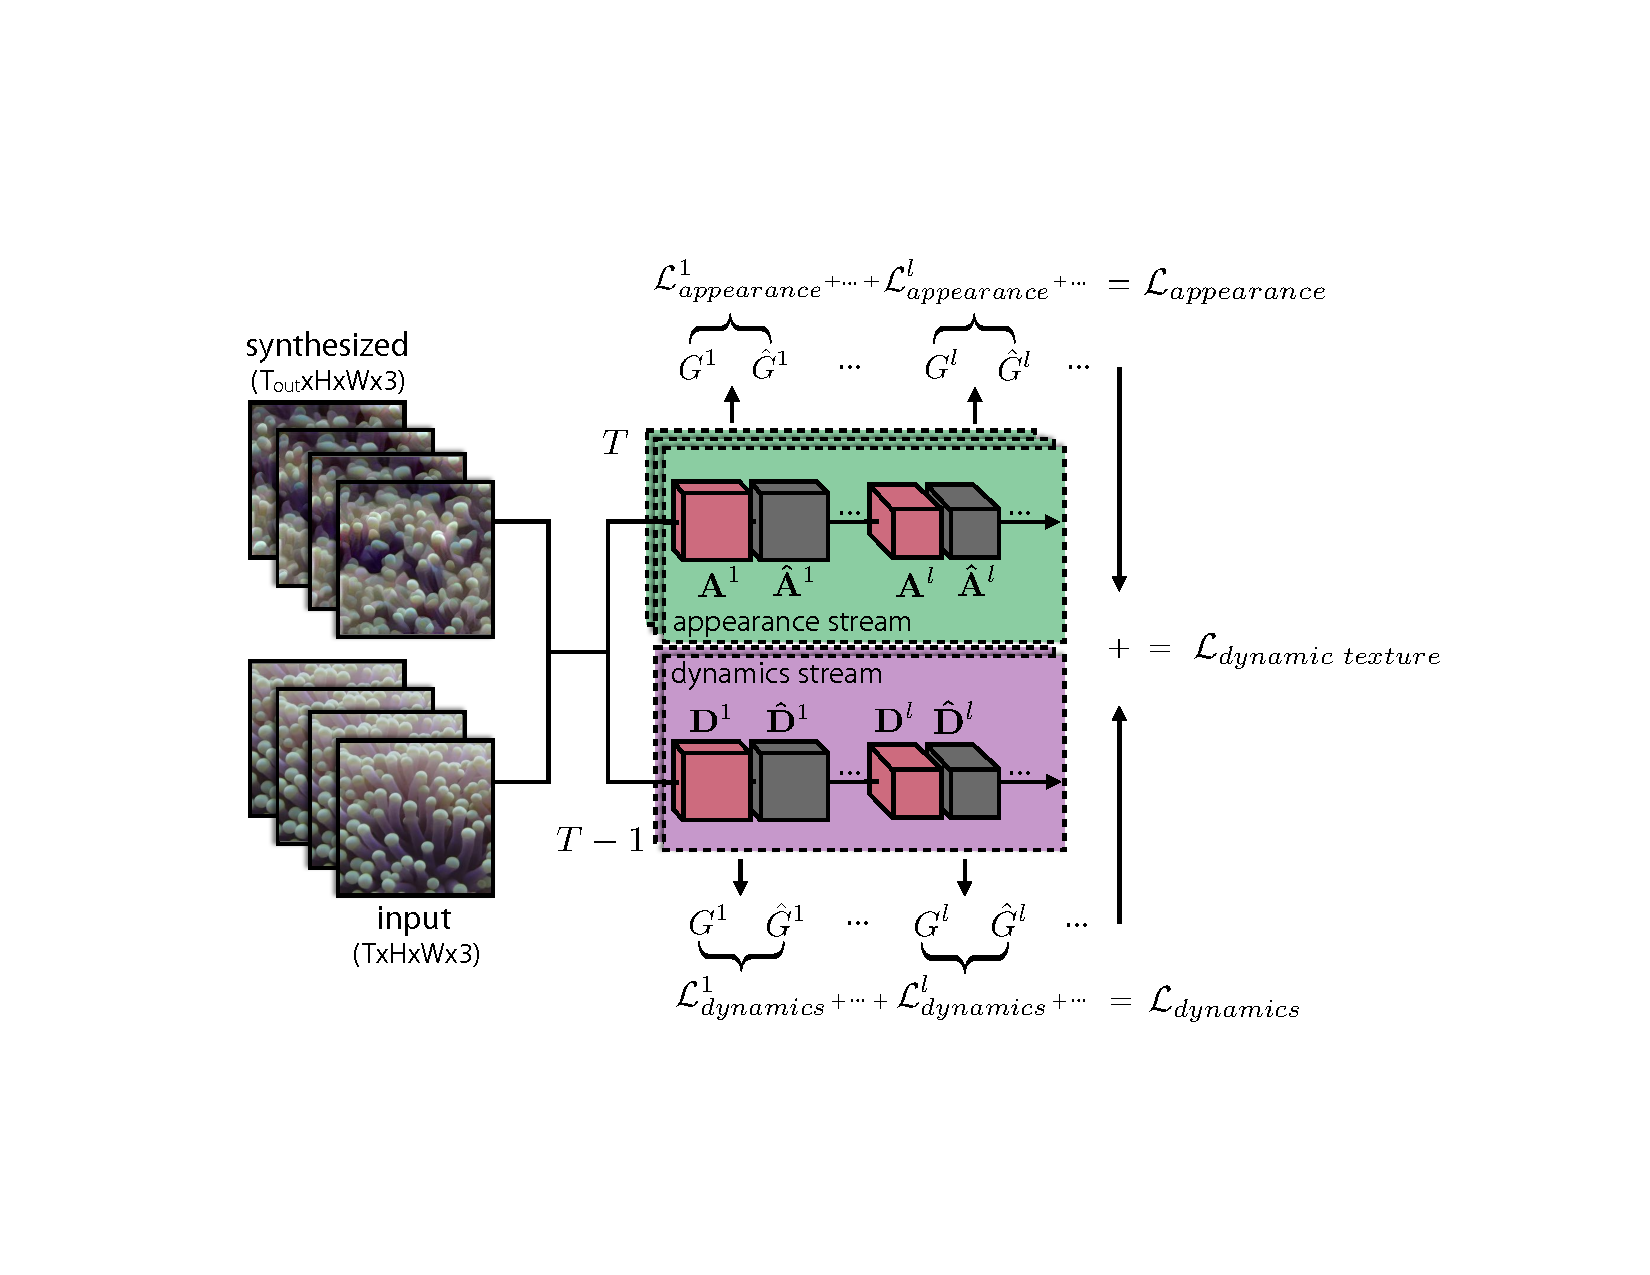
\epsfig{file=overallarchitecture.pdf, width = \textwidth}
\end{center}
\vspace{-0.45cm}
\caption[Two-stream dynamic texture generation.]{Two-stream dynamic texture generation.
Two sets of Gram matrices represent a dynamic texture's appearance and 
dynamics.
Matching these statistics allows for the generation of novel
textures as well as style transfer between textures. Here, $G^l$ and $\hat{G}^l$ are the Gram matrices of activations $A^l$ and $\hat{A}^l$ (or $D^l$ and $\hat{D}^l$) corresponding to the target and synthesized sequence, respectively, computed at layer $l$ of the appearance stream (or dynamics stream) and averaged over time $T$ (or $T-1$). $\mathcal{L}_\text{appearance}^l$ is the appearance loss at layer $l$, computed as the squared Frobenius norm between $G^l$ and $\hat{G}^l$ from the appearance stream. Similarly, $\mathcal{L}_\text{dynamics}^l$ is the dynamics loss at layer $l$ for the dynamics stream. By summing each loss computed at various layers, we arrive at $\mathcal{L}_\text{appearance}$ and $\mathcal{L}_\text{dynamics}$, which, when summed, form the combined dynamic texture loss, $\mathcal{L}_\text{dynamic texture}$, that is to be minimized.}
\label{fig:architecture}
\end{figure}


\section{Texture model: Appearance stream}

The appearance stream follows the spatial texture model
introduced by Gatys et al.\ \cite{gatys2015} which is
briefly reviewed here.
The key idea is that feature correlations in a 
ConvNet trained for 
object recognition  
capture texture appearance.
The same publicly available normalized VGG-19 network \cite{simonyan2014very} used by Gatys et al.\ \cite{gatys2015} is used here.

To capture the appearance of an input dynamic texture, we first
perform a forward pass with each frame of the image sequence
through the ConvNet and compute the feature activations,
$\mathbf{A}^{lt} \in \mathbb{R}^{N_l\times M_l}$, for various
levels in the network, where $N_l$ and $M_l$ denote
the number of filters and the number of spatial locations of layer
$l$ at time $t$, respectively.
The correlations of the filter responses in a particular layer are
averaged over the frames and encapsulated by a Gram matrix,
$\mathbf{G}^{l} \in \mathbb{R}^{N_l \times N_l}$, whose
entries are given by
$G_{ij}^l = \frac{1}{T N_l M_l} \sum_{t=1}^T \sum_{k=1}^{M_l} A_{ik}^{lt} A_{jk}^{lt}$,
where $T$ denotes the number of input frames
and $A_{ik}^{lt}$ denotes the activation of feature $i$ at
location $k$ in layer $l$ on the target frame $t$.
The synthesized texture appearance is similarly represented by a
Gram matrix, $\hat{\mathbf{G}}^{lt} \in \mathbb{R}^{N_l \times N_l}$,
whose activations are given by
$\hat{G}_{ij}^{lt} = \frac{1}{N_l M_l} \sum_{k=1}^{M_l} \hat{A}_{ik}^{lt} \hat{A}_{jk}^{lt}$,
where $\hat{A}_{ik}^{lt}$ denotes the activation of feature $i$ at
location $k$ in layer $l$ on the synthesized frame $t$.
The appearance loss, $\mathcal{L}_\text{appearance}$, is then 
defined as the temporal average of the mean squared error between
the Gram matrix of the input texture and that of the generated
texture computed at each frame:
\begin{equation}
   \mathcal{L}_\text{appearance} = \frac{1}{L_\text{app} T_\text{out}} \sum_{t=1}^{T_\text{out}} \sum_{l} \Vert \mathbf{G}^l - \hat{\mathbf{G}}^{lt} \Vert^2_F\ ,
   \label{eq:apploss}
\end{equation}
where $L_\text{app}$ is the number of layers used to compute Gram
matrices, $T_\text{out}$ is the number of frames being generated in
the output, and $\Vert \cdot \Vert_F$ is the Frobenius norm.
Consistent with previous work \cite{gatys2015}, we compute Gram matrices on the
following layers: 
\emph{conv1\_1}, \emph{pool1}, \emph{pool2}, \emph{pool3}, and \emph{pool4}.

\section{Texture model: Dynamics stream}

There are three primary goals in designing our dynamics stream.
First, the activations of the network must 
represent the temporal variation of the input pattern.
Second, the activations should be largely invariant to the
appearance of the images which should be characterized
by the appearance stream described above.
Finally, the representation must be differentiable to enable 
synthesis.
By analogy to the appearance stream, an obvious choice
is a ConvNet architecture suited for computing
optical flow (\eg, \cite{dosovitskiy2015,ilg2017}) which
is naturally differentiable.
However, with most such models it is unclear how invariant
their layers are to appearance.
Instead, we propose a novel network architecture which is
motivated by the spacetime-oriented energy model
\cite{derpanis2012spacetime,simoncelli1998}.

In motion energy models, the velocity of image content (\ie, motion)
is interpreted as a three-dimensional orientation in the $x$-$y$-$t$
spatiotemporal domain
\cite{adelson1985spatiotemporal,fahle1981,heeger1988,simoncelli1998,watson1983}.
In the frequency domain, the signal energy of a translating
pattern can be shown to lie on a plane through the origin
where the slant of the plane is defined by the velocity of
the  pattern.
Thus, motion energy models attempt to identify this 
orientation-plane (and hence the patterns velocity) via
a set of image filtering operations.
More generally
the constituent
spacetime orientations for a spectrum of common
visual patterns (including translation and dynamic
textures) can serve as a basis for describing the temporal
variation of an image sequence \cite{derpanis2012spacetime}.
This suggests that motion energy models may form an
ideal basis for our dynamics stream.

Specifically, we use the spacetime-oriented energy model
\cite{derpanis2012spacetime,simoncelli1998} to motivate our
network architecture which we briefly review here; 
see \cite{derpanis2012spacetime} for a more in-depth 
description.
Given an input video, 
a bank of oriented 3D
filters are applied which are sensitive to a range of
spatiotemporal orientations.
These filter activations are rectified (squared) and
pooled over local regions to make the responses robust
to the phase of the input signal, \ie, robust to the
alignment of the filter with the underlying image
structure.
Next, filter activations consistent with the same spacetime
orientation are summed.
These responses provide a pixelwise distributed measure
of which orientations (frequency domain planes) are
present in the input.
However, these responses are confounded by local image
contrast that makes 
it difficult to determine
whether a high response is indicative of the presence of
a spacetime orientation or simply due to high image
contrast.
To address this ambiguity, an $\textrm{L}_1$
normalization is applied across orientation responses which
results in a representation that is robust to local
appearance variations but highly selective to 
spacetime orientation.

Using this model as our basis, we propose the following 
fully convolutional 
network
\cite{shelhamer2017}.
Our ConvNet input is a pair of temporally consecutive greyscale images.
Each input pair is first normalized to have zero-mean and unit
variance.
This step provides a level of invariance to overall
brightness and contrast, \ie, global additive and
multiplicative signal variations.
The first layer consists of 32 3D spacetime convolution
filters of size $11\times 11 \times 2$
($\text{height} \times \text{width} \times \text{time}$).
Next, a squaring activation function and $5 \times 5$
spatial max-pooling (with a stride of one) is applied to
make the responses robust to local signal phase.
A $1\times 1$
convolution layer follows with 64 filters that combines
energy measurements that are consistent
with the same orientation.
Finally, to remove local contrast dependence, an
$\text{L}_1$ divisive normalization is applied.

To capture spacetime orientations beyond those capable
with the limited receptive fields used in the initial
layer, we compute a five-level spatial Gaussian pyramid.
Each pyramid level is
processed independently
with the same spacetime-oriented energy model and then
bilinearly upsampled to the original resolution and
concatenated.

Prior energy model instantiations (\eg,
\cite{adelson1985spatiotemporal,derpanis2012spacetime,simoncelli1998})
used handcrafted filter weights.
While a similar approach could be followed here, we
opt to learn the weights so that they are better
tuned to natural imagery.
To train the network weights, we add additional decoding
layers that take the concatenated distributed
representation and apply a $3\times 3$ convolution
(with 64 filters), ReLU activation, and a $1\times 1$
convolution (with 2 filters) that yields a two channel
output encoding the optical flow directly.
The proposed architecture is illustrated in
Fig.\ \ref{fig:MSOE}.

\begin{figure}[t]
\begin{center}
    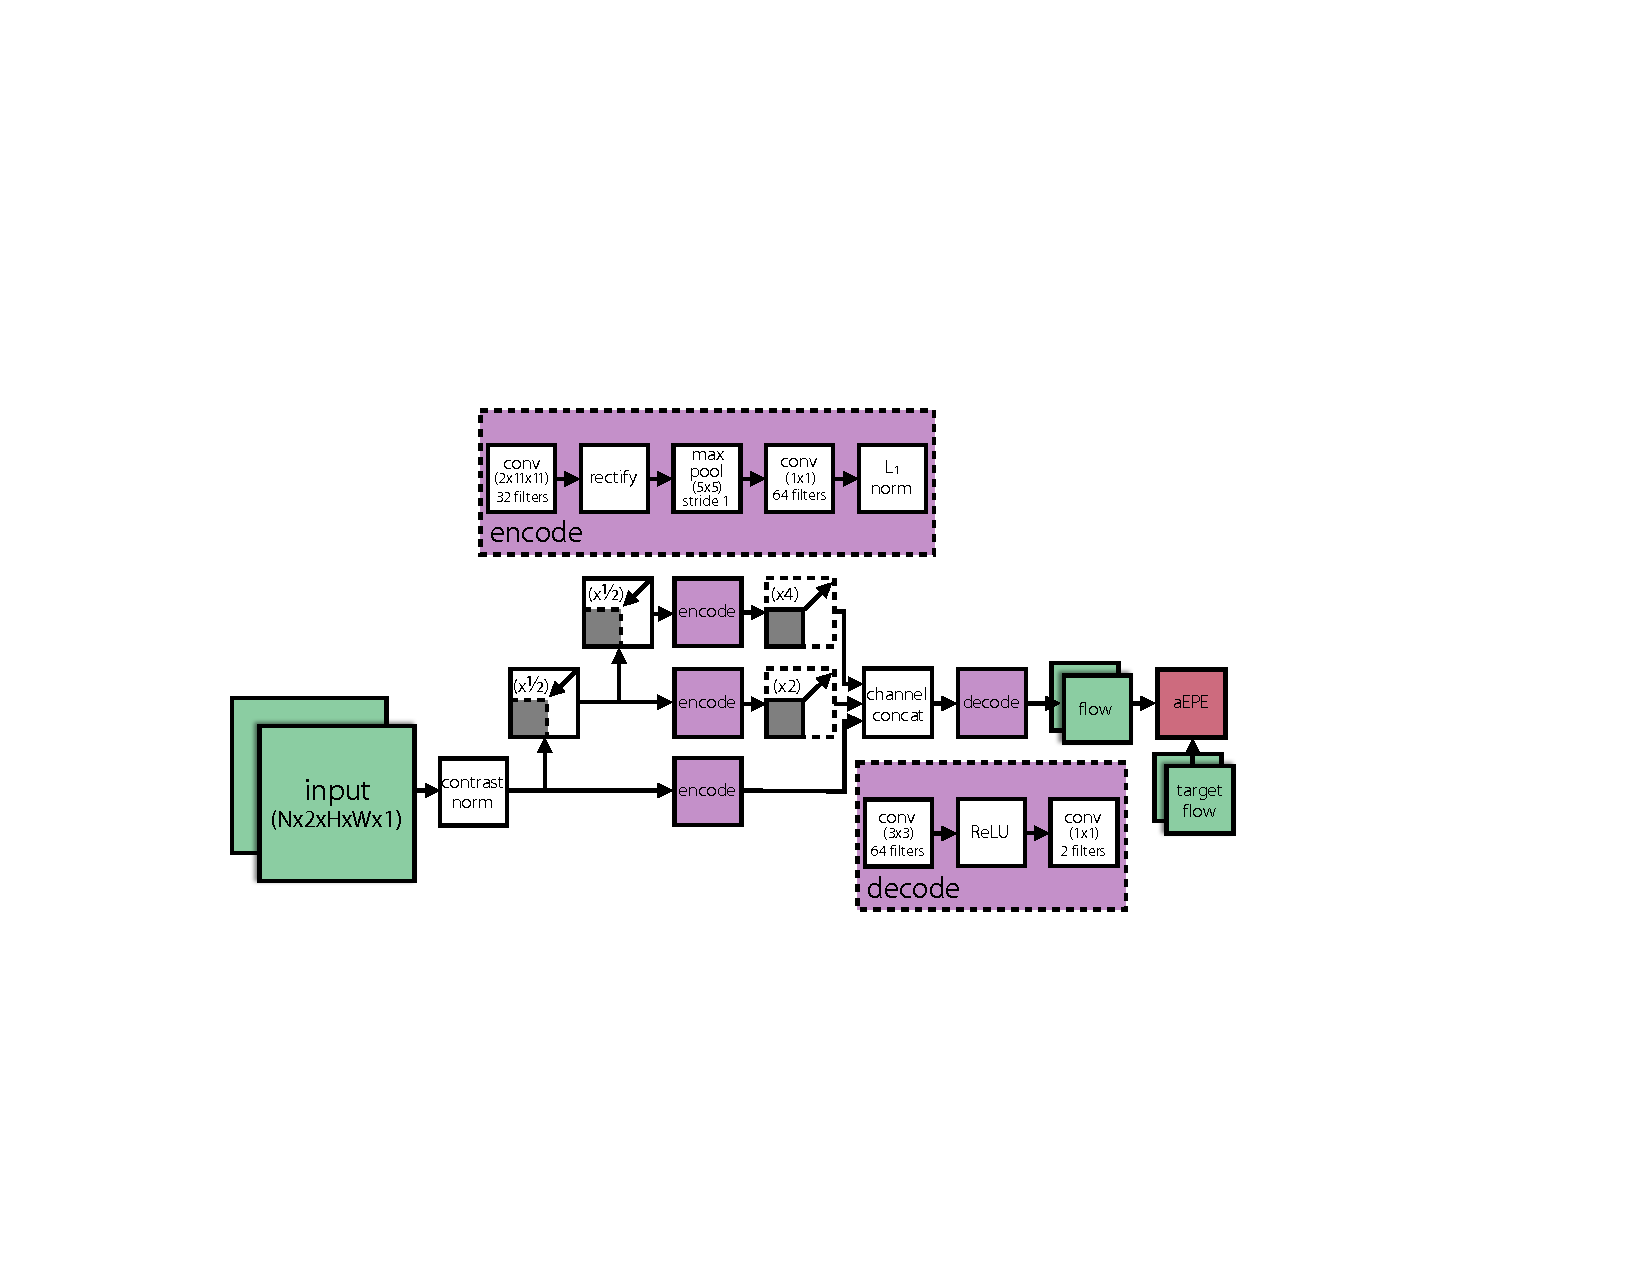
\epsfig{file=MSOEnet.pdf, width = \textwidth}
\end{center}
\vspace{-0.45cm}
\caption[Dynamics stream ConvNet.]{Dynamics stream ConvNet. The ConvNet is based on a
spacetime-oriented energy model
\cite{derpanis2012spacetime, simoncelli1998} and is trained
for optical flow prediction.
Three scales are shown for illustration;
in practice five scales are used.}
\label{fig:MSOE}
\end{figure}

For training, we use the standard average
endpoint error (aEPE) flow metric (\ie, $\text{L}_2$
norm) between the predicted flow and the ground truth
flow as the loss.
Since no large-scale flow dataset exists that captures
natural imagery with groundtruth flow, we take an
unlabeled video dataset and apply an existing flow
estimator \cite{revaud2015epicflow} to estimate optical
flow for training,
\cf \cite{tran2016}.
For training data, we used videos from the UCF101
dataset \cite{soomro2012ucf101} with geometric
and photometric data augmentations similar to those used
by FlowNet \cite{dosovitskiy2015}, and optimized the aEPE loss using
Adam \cite{kingma2017}.
Inspection of the learned filters in the initial layer
showed evidence of spacetime-oriented filters, consistent with
the handcrafted filters used in previous work \cite{derpanis2012spacetime}.

Similar to the appearance stream, filter response correlations
in a particular layer of the dynamics
stream are averaged over the number of image frame
pairs and encapsulated by a Gram matrix,
$\mathbf{G}^{l} \in \mathbb{R}^{N_l \times N_l}$,
whose entries are given by
$G_{ij}^l = \frac{1}{(T-1) N_l M_l} \sum_{t=1}^{T-1} \sum_{k=1}^{M_l} D_{ik}^{lt} D_{jk}^{lt}$,
where $D_{ik}^{lt}$ denotes the activation of feature $i$ at
location $k$ in layer $l$ on the target frames $t$ and $t+1$.
The dynamics of the synthesized texture is represented
by a Gram matrix of filter response correlations 
computed separately for each pair of frames,
$\hat{\mathbf{G}}^{lt} \in \mathbb{R}^{N_l \times N_l}$,
with entries
$\hat{G}_{ij}^{lt} = \frac{1}{N_l M_l} \sum_{k=1}^{M_l} \hat{D}_{ik}^{lt} \hat{D}_{jk}^{lt}$,
where $\hat{D}_{ik}^{lt}$ denotes the activation of feature $i$ at
location $k$ in layer $l$ on the synthesized frames $t$ and $t+1$.
The dynamics loss, $\mathcal{L}_\text{dynamics}$, is defined as
the average of the mean squared error between the Gram matrices
of the input texture
and those of the generated texture:
\begin{equation}
   \mathcal{L}_\text{dynamics} = \frac{1}{L_\text{dyn} (T_\text{out}-1)}\sum_{t=1}^{T_\text{out}-1} \sum_{l}  \Vert \mathbf{G}^l - \hat{\mathbf{G}}^{lt}\Vert^2_F, \label{eq:dynloss}
\end{equation}
where $L_\text{dyn}$ is the number of ConvNet layers being used
in the dynamics stream.

Here we propose to use the output of the concatenation layer,
where the multiscale distributed representation of orientations is
stored, as the layer to compute the Gram matrix.
While it is tempting to use the predicted flow output from the
network, this generally yields poor results as shown in our evaluation.
Due to the complex, temporal variation present in dynamic
textures, they contain a variety of local spacetime
orientations rather than a single dominant orientation.
As a result, the flow estimates will tend to be an average of the
underlying  orientation measurements and consequently not
descriptive. A comparison between the texture synthesis results using the concatenation layer and the predicted flow output is provided in Sec.\ \ref{empirical_evaluation}.

\section{Texture generation}\label{sec:texgen}
The overall dynamic texture loss consists of the combination of the appearance loss, Eq.\ (\ref{eq:apploss}),
and the dynamics loss, Eq.\ (\ref{eq:dynloss}):
\begin{equation}
   \mathcal{L}_\text{dynamic texture} = \alpha\mathcal{L}_\text{appearance} + \beta \mathcal{L}_\text{dynamics}, \label{eq:dyntexloss}
\end{equation}
where $\alpha$ and $\beta$ are the weighting factors for the
appearance and dynamics content, respectively.
Dynamic textures are implicitly defined as the (local) minima 
of this loss.
Textures are generated by optimizing Eq.\ 
(\ref{eq:dyntexloss}) with respect to the spacetime volume,
\ie, the pixels of the video.
Variations in the resulting texture are found by initializing the
optimization process using IID Gaussian noise.
Consistent with previous work \cite{gatys2015}, we use
L-BFGS \cite{liu1989} optimization. 

Naive application of the outlined approach will consume
increasing amounts of memory as the temporal extent of the 
dynamic texture grows; this makes it impractical to generate
longer sequences.
Instead, long sequences can be incrementally generated by
separating the sequence into subsequences and optimizing them 
sequentially.  This is realized by initializing the first frame of a subsequence as the last 
frame from the previous subsequence and keeping it fixed throughout
the optimization.
The remaining frames of the subsequence are initialized randomly and
optimized as above.
This ensures temporal consistency across synthesized subsequences
and can be viewed as a form of coordinate descent for the full
sequence objective.
The flexibility of this framework allows other texture generation
problems to be handled simply by altering the 
initialization of frames and controlling which
frames or frame regions are updated.

\chapter{Evaluation}\label{chap:evaluation}

The goal of (dynamic) texture synthesis is to generate 
samples that are indistinguishable from the real input target
texture by a human observer.
In this chapter, a variety of synthesis results are presented,
including qualitative comparisons with extant methods and a user study to quantitatively evaluate the realism
of the synthesized results.
Given their temporal nature, the results are best viewed as 
videos, which are available on the project page: \url{ryersonvisionlab.github.io/two-stream-projpage}.
The two-stream architecture was implemented using TensorFlow
\cite{tabadi2015tensorflow}, an open source machine learning framework.
Results were synthesized using an NVIDIA Titan X (Pascal) GPU
and synthesis times ranged between one to three hours (corresponding to $6,000$ optimization iterations)
to generate $12$ frames with an image resolution of 
$256 \times 256$. The parameters of the dynamics stream were set as follows: $\alpha = 1\mathrm{e}{9}$, $\beta = 1\mathrm{e}{15}$, $\epsilon = 1\mathrm{e}{-12}$, and $\eta = 1\mathrm{e}{-12}$.
For the full synthesis results and source code, please refer to the
supplemental material available on the project page.

\section{Qualitative results}\label{sec:qualitative_results}

In this section, a qualitative analysis is performed on the tasks of dynamic texture synthesis, incremental texture synthesis,
temporally-endless texture synthesis, and dynamics style transfer.

\subsection{Dynamic texture synthesis}

The dynamic texture synthesis process was applied 
to a wide range of textures selected from the 
DynTex \cite{peteri2010} database and others that were collected in-the-wild.
The collected textures include ones that adhere to the texture assumptions of this thesis (\ie, spatiotemporal homogeneity) and ones that do not.
Included in the supplemental material are synthesized results
of nearly 60 different textures that encapsulate a range of
phenomena, such as flowing water, waves, clouds, fire, rippling
flags, waving plants, and schools of fish.
Some sample frames are shown in Fig.\ \ref{fig:successes_1} and Fig.\ \ref{fig:successes_2}
but readers are encouraged to view the videos to fully appreciate
the results.

Figure \ref{fig:successes_1} and Fig.\ \ref{fig:successes_2} show some example success cases with the
two-stream method where appearance and dynamics characteristics from the
target are reliably preserved in the synthesized result. For example, the
upward fiery dynamics and flickering appearance of \path{fireplace_1}, the outward dynamics of the explosive splash of \path{lava},
the wispy fluid dynamics of \path{smoke_1}, the
flowing vegetation in \path{underwater_vegetation_1}, and the downward 
rippling flow of \path{water_3}, are all captured in the synthesized results.

\clearpage
\begin{figure*}[t!]
\begin{center}
\begin{tabular}{ >{\centering\arraybackslash} m{0.16\textwidth} || >{\centering\arraybackslash} m{0.80\textwidth} }

{\footnotesize \path{fireplace_1}\break(original)} &
\showtexture{fireplace_1/frame_} \\
\hline
{\footnotesize \path{fireplace_1}\break(synthesized)} &
\showtexture{fireplace_1_output/frame_} \\

\hline \hline
{\footnotesize \path{lava}\break(original)} &
\showtexture{lava/frame_} \\
\hline
{\footnotesize \path{lava}\break(synthesized)} &
\showtexture{lava_output/frame_} \\

\hline \hline
{\footnotesize \path{smoke_1}\break(original)} &
\showtexture{smoke_1/frame_} \\
\hline
{\footnotesize \path{smoke_1}\break(synthesized)} &
\showtexture{smoke_1_output/frame_} \\

%\hline \hline
%{\footnotesize \path{underwater_vegetation_1}\break(original)} &
%\showtexture{underwater_vegetation/frame_} \\
%\hline
%{\footnotesize \path{underwater_vegetation_1}\break (synthesized)} &
%\showtexture{underwater_vegetation_output/frame_} \\
%
%\hline \hline
%{\footnotesize \path{water_3}\break(original)} & 
%\showtexture{water_3/frame_} \\
%\hline
%{\footnotesize \path{water_3}\break(synthesized)} & 
%\showtexture{water_3_output/frame_} \\
\end{tabular}
\end{center}
\vspace{-0.45cm}
\caption[Dynamic texture synthesis success examples]{Dynamic texture synthesis success examples. Names correspond to files in the supplemental material.}
 \label{fig:successes_1}
\end{figure*}

\begin{figure*}[t!]
\begin{center}
\begin{tabular}{ >{\centering\arraybackslash} m{0.16\textwidth} || >{\centering\arraybackslash} m{0.80\textwidth} }
{\footnotesize \path{underwater_vegetation_1}\break(original)} &
\showtexture{underwater_vegetation/frame_} \\
\hline
{\footnotesize \path{underwater_vegetation_1}\break (synthesized)} &
\showtexture{underwater_vegetation_output/frame_} \\

\hline \hline
{\footnotesize \path{water_3}\break(original)} & 
\showtexture{water_3/frame_} \\
\hline
{\footnotesize \path{water_3}\break(synthesized)} & 
\showtexture{water_3_output/frame_} \\
\end{tabular}
\end{center}
\vspace{-0.45cm}
\caption[Dynamic texture synthesis success examples]{Dynamic texture synthesis success examples. Names correspond to files in the supplemental material.}
 \label{fig:successes_2}
\end{figure*}

\clearpage

\subsubsection{Failure modes}

Example failure modes of the two-stream method are presented in Fig.\ 
\ref{fig:failures}.
In general, most failures result from inputs that
violate the underlying assumption of a dynamic texture, \ie, 
the appearance and/or dynamics are not spatiotemporally homogeneous.
In the case of the \path{escalator} example, the long edge 
structures in the appearance are not spatially homogeneous, 
and the dynamics vary due to perspective effects that
change the motion from purely downward to downward and outward.
The resulting synthesized texture captures an overall downward 
motion but lacks the perspective effects and is unable to 
consistently reproduce the long edge structures.
This is consistent with previous observations
on static texture synthesis \cite{gatys2015} and suggests it is a 
limitation of the Gram matrix representation used
in the appearance stream.

Another example is the \path{flag} sequence where the rippling 
dynamics are relatively homogeneous across the pattern but the 
appearance varies spatially.
As expected, the synthesized texture does not faithfully
reproduce the appearance; however, it does exhibit plausible 
rippling dynamics.

Also shown in Fig.\ \ref{fig:failures} is the \path{cranberries} sequence, which consists of a combination of swirling and wave dynamics.
The model faithfully reproduces the appearance
but is unable to capture the spatially varying dynamics.
Interestingly, it still produces a result
which is statistically indistinguishable from real in the user 
study discussed in Sec.\ \ref{sec:user_study}.

\clearpage
\begin{figure}[t]
\begin{center}
\begin{tabular}{ >{\centering\arraybackslash} m{0.16\textwidth} || >{\centering\arraybackslash} m{0.80\textwidth} }
{\footnotesize \path{escalator}\break(original)} & 
\showtexture{escalator/frame_} \\
\hline
{\footnotesize \path{escalator}\break(synthesized)} & 
\showtexture{escalator_output/frame_} \\
\hline \hline
{\footnotesize \path{flag}\break(original)} &
\showtexture{flag/frame_} \\
\hline
{\footnotesize \path{flag}\break(synthesized)} &
\showtexture{flag_output/frame_} \\
\hline \hline
{\footnotesize \path{cranberries}\break(original)} &
\showtexture{cranberries/frame_} \\
\hline
{\footnotesize \path{cranberries}\break(synthesized)} &
\showtexture{cranberries_output/frame_} \\
\end{tabular}
\end{center}
\vspace{-0.45cm}
\caption[Dynamic texture synthesis failure examples.]{Dynamic texture synthesis failure examples. In
these cases, the failures are attributed to either the
appearance or the dynamics not being homogeneous.}
\label{fig:failures}
\end{figure}
\clearpage

\subsubsection{Appearance vs.\ dynamics streams}

Two experiments were conducted to verify that the appearance and dynamics
streams were capturing complementary information.
To validate that the texture generation of multiple frames
would not induce dynamics consistent with the input, frames were synthesized
starting from randomly generated noise but only using the
appearance statistics and corresponding loss, \ie,
Eq.\ \ref{eq:apploss}.
As expected, this produced frames that were valid textures but
with no coherent dynamics present.
To examine the dynamics, see 
\path{fish} in the supplemental material.

Similarly, to validate that the dynamics stream did not 
inadvertently include appearance information, dynamic textures were synthesized
using the dynamics loss only, \ie, Eq.\ \ref{eq:dynloss}.
The resulting frames had no visible appearance and had
an extremely low dynamic range, \ie, the standard
deviation of pixel intensities was 10 for values in $[0,255]$.
This indicates a general invariance to appearance and 
suggests that the two-stream dynamic texture representation
has factored appearance and dynamics, as desired.
Results for a sequence containing a school of fish are shown in
Fig.\ \ref{fig:appearance_only_vs_dynamics_only} with enhanced contrast.

\begin{figure}[t]
\begin{center}
\begin{tabular}{ >{\centering\arraybackslash} m{0.16\textwidth} || >{\centering\arraybackslash} m{0.80\textwidth} }
{target (\path{fish})} & 
\showtexture{fish/frame_} \\
\hline \hline
{appearance only} &
\showtexture{fish_spatialonly/frame_} \\
\hline
{dynamics only} &
\showtexture{fish_dynamicsonly/frame_} \\
\hline
{both streams} & 
\showtexture{fish_output/frame_} \\
\end{tabular}
\end{center}
\vspace{-0.45cm}
\caption[Two-stream dynamic texture synthesis versus dynamics-only and appearance-only texture synthesis]{Two-stream dynamic texture synthesis versus dynamics-only and appearance-only texture synthesis.
(top row) Target dynamic texture.
(second row)
Texture synthesis without dynamics constraints shows
consistent per-frame appearance but no temporal coherence.
(third row)
Texture synthesis without appearance constraints shows
limited per-frame appearance with pixel intensities having a standard deviation of 10.
(bottom row)
Including both streams induces consistent appearance and dynamics.
}
\label{fig:appearance_only_vs_dynamics_only}
\end{figure}



\subsection{Incremental texture synthesis}

Dynamic textures synthesized incrementally, as described in Sec.\
\ref{sec:incremental_synthesis}, are included in the supplemental.
Sequences as long as 122 frames (using 11 frame subsequences) were synthesized
with no observed divergence or degradation. The resulting textures were 
perceptually indistinguishable from those synthesized with the typical batch process.

\subsection{Temporally-endless texture synthesis}

An example of a synthesized temporally-endless dynamic texture is shown in
Fig.\ \ref{fig:temporally_endless_synthesis}. As described in Sec.\ 
\ref{sec:temporally_endless_synthesis}, the dynamic texture appears
temporally endless, \ie, there is no apparent temporal discontinuity between the last and first frames.

\begin{figure}[t]
	\centering
    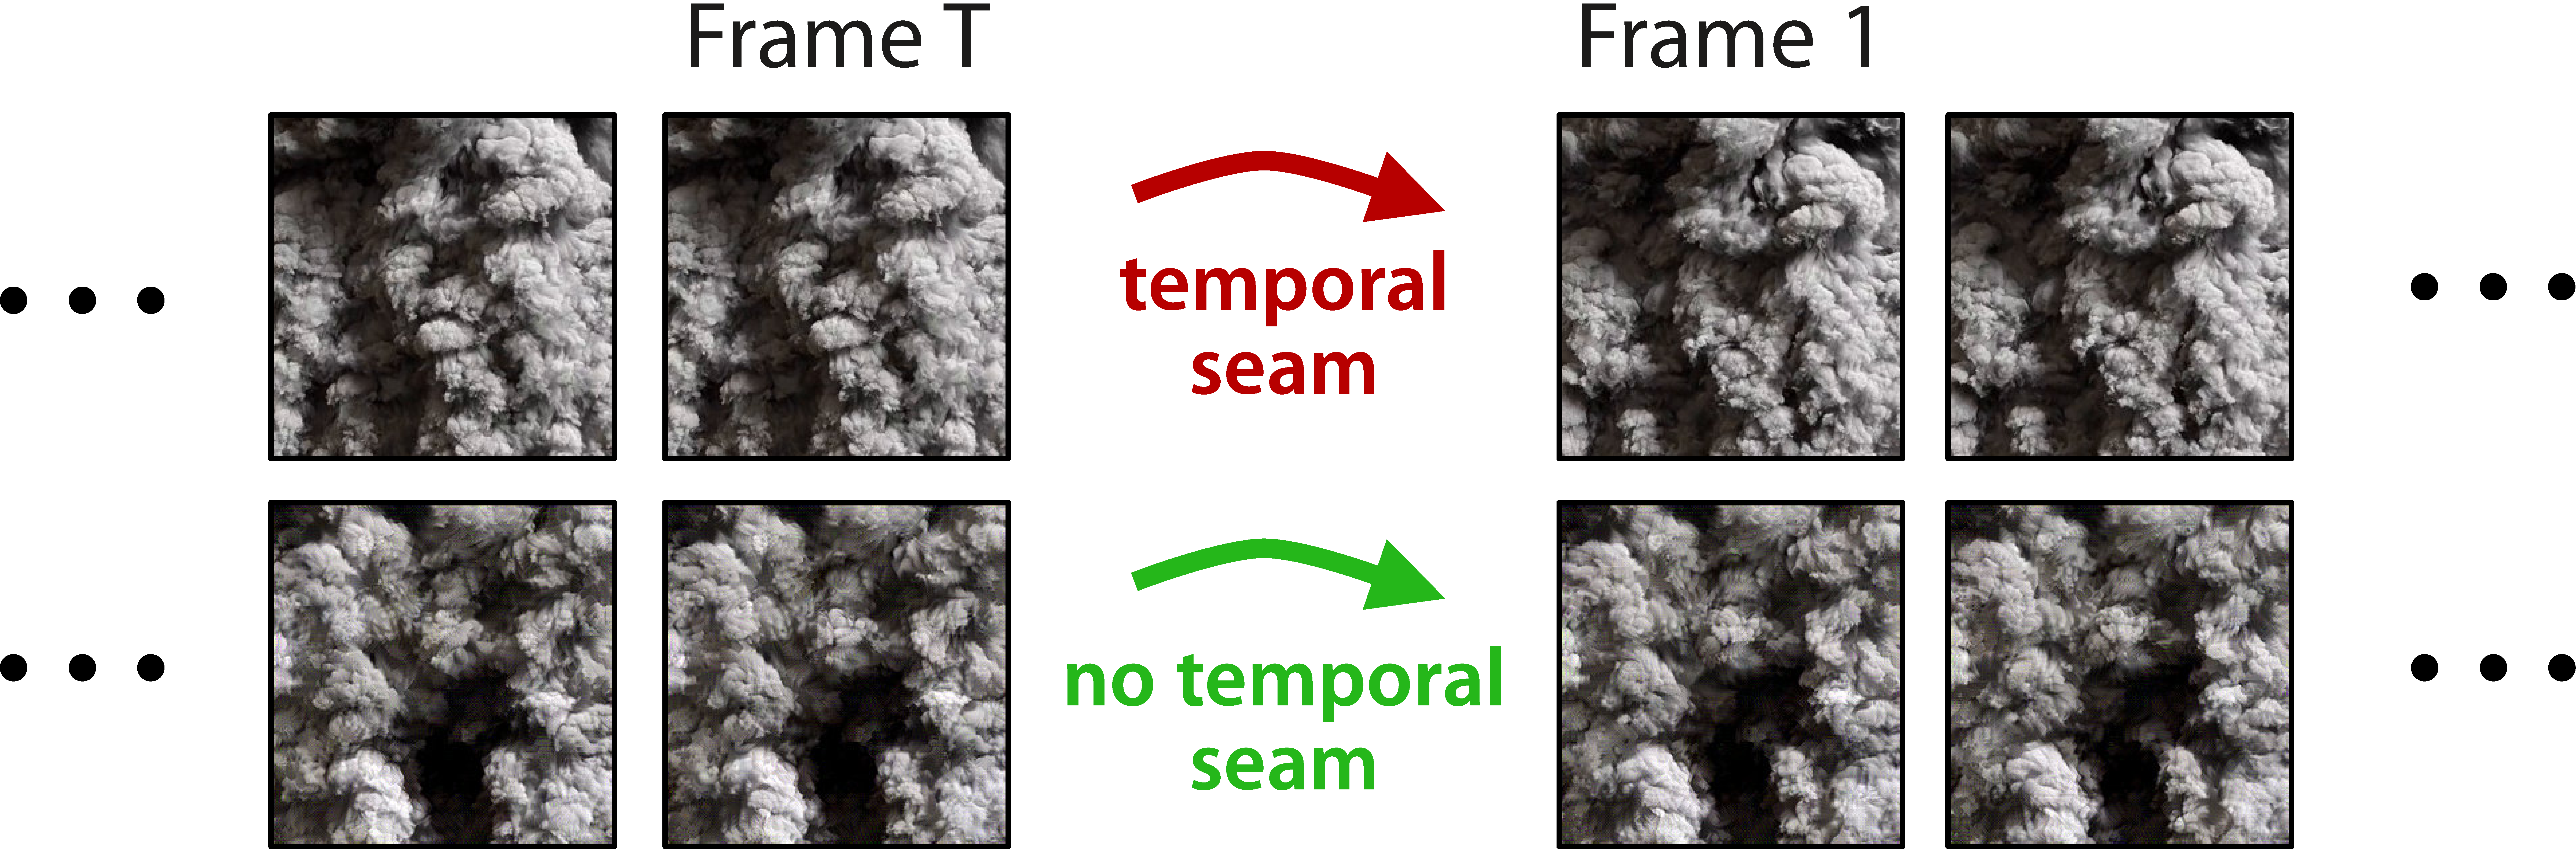
\epsfig{file=temporally_endless_synthesis.pdf, width = 0.9\textwidth}
	\caption[Temporally-endless texture synthesis.]{Temporally-endless texture synthesis. (top row) Target texture. (bottom row) Synthesized texture.
	 By adding an additional loss to the dynamics stream that ties the last frame to the first, the synthesized dynamic texture appears to be temporally endless. Note the lack of an abrupt appearance change (\ie, temporal seam) between the last frame and the first frame of the synthesized dynamic texture.}
	\label{fig:temporally_endless_synthesis}
\end{figure}



\subsection{Dynamics style transfer}

A dynamics style transfer results is shown in Fig.\ 
\ref{fig:motiontransfer} (top row), using two real videos as the appearance and dynamics target, respectively.
Additional examples are available in the supplemental material.
When performing dynamics style transfer it is important
that the appearance structure of both targets to be similar in scale and semantics,
otherwise, the synthesized dynamic textures will look unnatural.
For instance, transferring the dynamics of a flame onto a water 
scene will generally produce implausible results (Fig.\ \ref{fig:bad_motiontransfer}).

\begin{figure}[t]
\begin{center}
\begin{tabular}{>{\centering\arraybackslash} m{0.16\textwidth} || >{\centering\arraybackslash} m{0.80\textwidth} }
appearance target &
synthesized output \\
\hline \hline
\vspace{0.1cm}\showtexframe{water_paint.jpeg} &
\showtexture{fireplace_1_to_water_paint_output/frame_} \\
\end{tabular}
\end{center}
\vspace{-0.45cm}
\caption[Dynamics style transfer with incompatible appearance and dynamics targets]{Dynamics style transfer with incompatible appearance and dynamics targets. The dynamics from \path{fireplace_1} are unsuccessfully transferred to a painting of ocean water.}
\label{fig:bad_motiontransfer}
\end{figure}



The dynamics of a texture can also be applied to a static input image,
as the target Gram matrices for the appearance loss can be computed
on just a single frame.
This allows us to effectively animate regions of a static image.
The result of this process can be striking and is visualized in
Fig.\ \ref{fig:motiontransfer} (second, third, and bottom rows), where the appearance is 
taken from a painting and the dynamics from a real world video.

\clearpage
\begin{figure}[t]
\begin{center}
\begin{tabular}{ >{\centering\arraybackslash} m{0.16\textwidth} || >{\centering\arraybackslash} m{0.80\textwidth} }
appearance target &
synthesized output \\
\hline \hline
\vspace{0.1cm}\showtexframe{water_img.jpeg} &
\showtexture{water_4_to_water_img_output/frame_} \\
\hline
\vspace{0.1cm}\showtexframe{fire_paint.jpeg} &
\showtexture{fireplace_1_to_fire_paint_output/frame_} \\
\end{tabular}
\end{center}
\vspace{-0.45cm}
\caption[Dynamics style transfer.]{Dynamics style transfer.
(top row) 
Appearance of still water was
used with the dynamics of a different water dynamic texture
(\path{water_4}).
(bottom row) 
The appearance of a painting of fire was used
with the dynamics of a real fire (\path{fireplace_1}).
Animated results and additional examples are available in
the supplemental material.} 
\label{fig:motiontransfer}
\end{figure}
\clearpage

\section{User study}\label{sec:user_study}

Quantitative evaluation for (dynamic) texture synthesis is a particularly
challenging task as there is no single correct output when 
synthesizing new samples of a texture.
Like in other image generation tasks (\eg, rendering), 
human perception is ultimately the most important measure.
Thus, a user study was performed to evaluate the perceived 
realism of the synthesized dynamic textures.

Similar to previous image synthesis work (\eg, \cite{chen2017}), 
a perceptual experiment was conducted with human observers to 
quantitatively evaluate the synthesis results.
A two-way alternative forced-choice (2AFC) evaluation was employed on Amazon Mechanical
Turk (AMT) with 200 different users. Each user performed 59
pairwise comparisons between a synthesized dynamic texture and 
its target.
Users were asked to choose which dynamic texture appeared more realistic
after viewing the textures independently (with a brief delay between viewing each texture) for an exposure time sampled
randomly from discrete intervals between 0.3 and 4.8 seconds.
Measures were taken to control the experimental conditions and
minimize the possibility of low quality data.
Appendix \ref{sec:experimental_procedure} provides further experimental
details of the user study.

For comparison, a baseline was constructed by using the 
flow decode layer in the dynamics loss of Eq.\ \ref{eq:dynloss}.
This approach corresponds with attempting to mimic the optical flow 
statistics of the texture directly.
Textures were synthesized with this model and the user study
was repeated with an additional 200 users.
To differentiate between the models, ``Flow decode layer'' 
and ``Concat layer'' are labelled in the figures to describe the
baseline and final model, respectively. An example comparing a dynamic texture synthesized on the baseline and final model is shown in Fig.\ \ref{fig:baseline_comparison}.

\begin{figure}[t]
\begin{center}
\begin{tabular}{ >{\centering\arraybackslash} m{0.16\textwidth} || >{\centering\arraybackslash} m{0.80\textwidth} }
{target (\path{waterfall})} & 
\showtexture{waterfall/frame_} \\
\hline \hline
{flow decode layer (baseline)} &
\showtexture{waterfall_flowdecode/frame_} \\
\hline
{concatenation layer (final)} & 
\showtexture{waterfall_concat/frame_} \\
\end{tabular}
\end{center}
\vspace{-0.45cm}
\caption[Comparison with a dynamic texture synthesized using optical-flow directly]{Comparison with a dynamic texture synthesized using optical-flow directly.
(top row) Target dynamic texture.
(middle row)
Dynamic texture synthesis when using the ``Flow decode layer'' on the dynamics stream. This is the baseline model and corresponds to attempting to mimic the optical flow statistics of the texture directly. The dynamics of the waterfall are poorly captured, lacking the downward motion exhibited by the target.
(bottom row)
Dynamic texture synthesis when using the ``Concat layer'' on the dynamics stream. This is the final model. The downward motion and overall dynamics of the target are reliably captured.
}
\label{fig:baseline_comparison}
\end{figure}



The results of this study are summarized in
Fig.\ \ref{fig:pairwise_alltextures} which shows user accuracy in
differentiating real versus synthesized textures as a function of
time for both methods. Accuracies are reported with a $95\%$ confidence level, \ie, a margin of error that is between $\pm 1.96$ standard deviations from the mean ($p$-value of $0.05$).
Overall, users are able to correctly identify the real texture
$66.1\% \pm 2.5\%$ of the time for brief 
exposures of 0.3 seconds.
This rises to $79.6\% \pm 1.1\%$ with exposures of 1.2 seconds 
and higher.
Note that ``perfect'' synthesis results would have an accuracy
of $50\%$, indicating that users were unable to differentiate 
between the real and synthesized textures and higher accuracy 
indicating less convincing textures.

\begin{figure}[t]
	\centering
    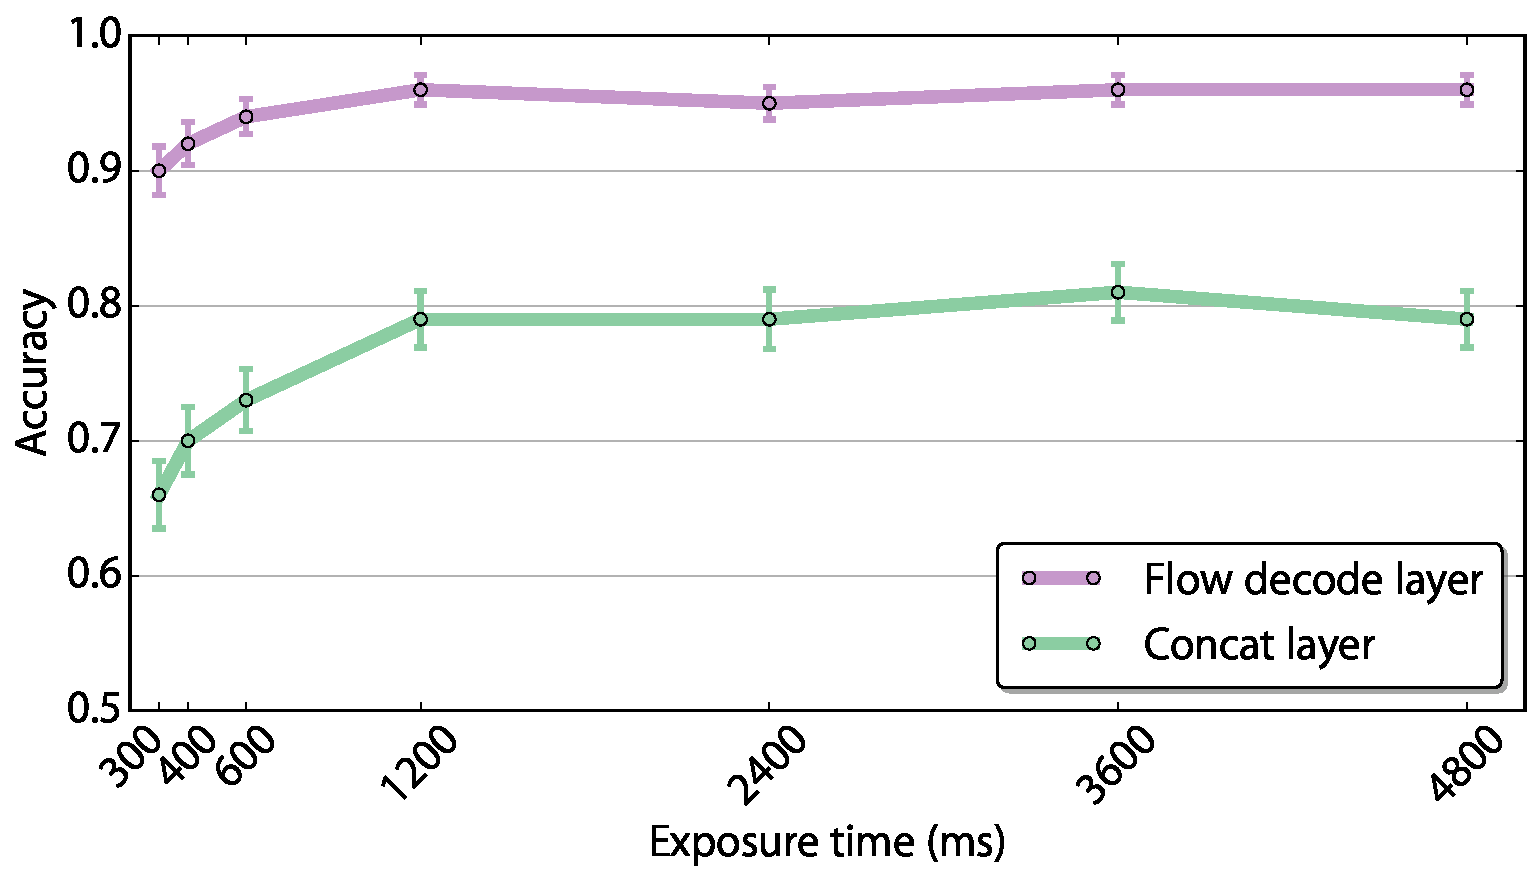
\epsfig{file=alltextures_approvedworkers.pdf, width = 0.9\textwidth}
	\caption[Time-limited pairwise comparisons across all textures]{Time-limited pairwise comparisons across all textures with $95\%$ statistical confidence intervals.}
	\label{fig:pairwise_alltextures}
\end{figure}



The results clearly show that the use of the concatenation 
layer's activations is far more effective than the flow decode 
layer.
This is not surprising, as optical flow alone is known to be 
unreliable on many textures, particularly those with
translucent and/or chaotic dynamics (\eg, water, smoke, flames, etc.). Specifically, its assumptions of a single coherent movement for each pixel and brightness constancy are violated.
Also evident in these results is the time-dependant nature of 
perception for textures from both models.
Users' ability to identify the synthesized texture improved as 
exposure times increased to 1.2 seconds and remained relatively 
flat for longer exposures.

To better understand the performance of the proposed approach,
the results were grouped and analyzed in terms of
appearance and dynamics characteristics.
For appearance, the taxonomy
presented in \cite{lin2006quantitative} was used to group textures as
either regular/near-regular (\eg, periodic tiling and brick wall), 
irregular (\eg, a field of flowers), or
stochastic/near-stochastic (\eg, tv static or water).
For dynamics, the textures were grouped as either 
spatially-consistent (\eg, closeup of rippling sea water) or 
spatially-inconsistent (\eg, rippling sea water viewed at an angle, causing inconsistent dynamics due to perspective distortion). The finer-grained dynamics taxonomy presented by Derpanis and Wildes \cite{derpanis2012spacetime} was not used here in its entirety because certain categories of dynamics were under-represented in the database of collected dynamic textures, \eg, unconstrained and underconstrained dynamics. Furthermore, there were dynamic textures that were difficult to categorize under their taxonomy (\ie, dynamic textures with inconsistent dynamics). To maintain statistically-meaningful results, the dominant, multi-dominant, heterogeneous, and isotropic dynamics groups of Derpanis and Wildes \cite{derpanis2012spacetime} were merged into the spatially-consistent group, covering roughly half of the collected dynamic textures, and the spatially-inconsistent group was created to cover the rest.
Results based on these groupings can be seen in
Fig.\ \ref{fig:pairwise_grouped}.

\begin{figure}[t]
	\centering
	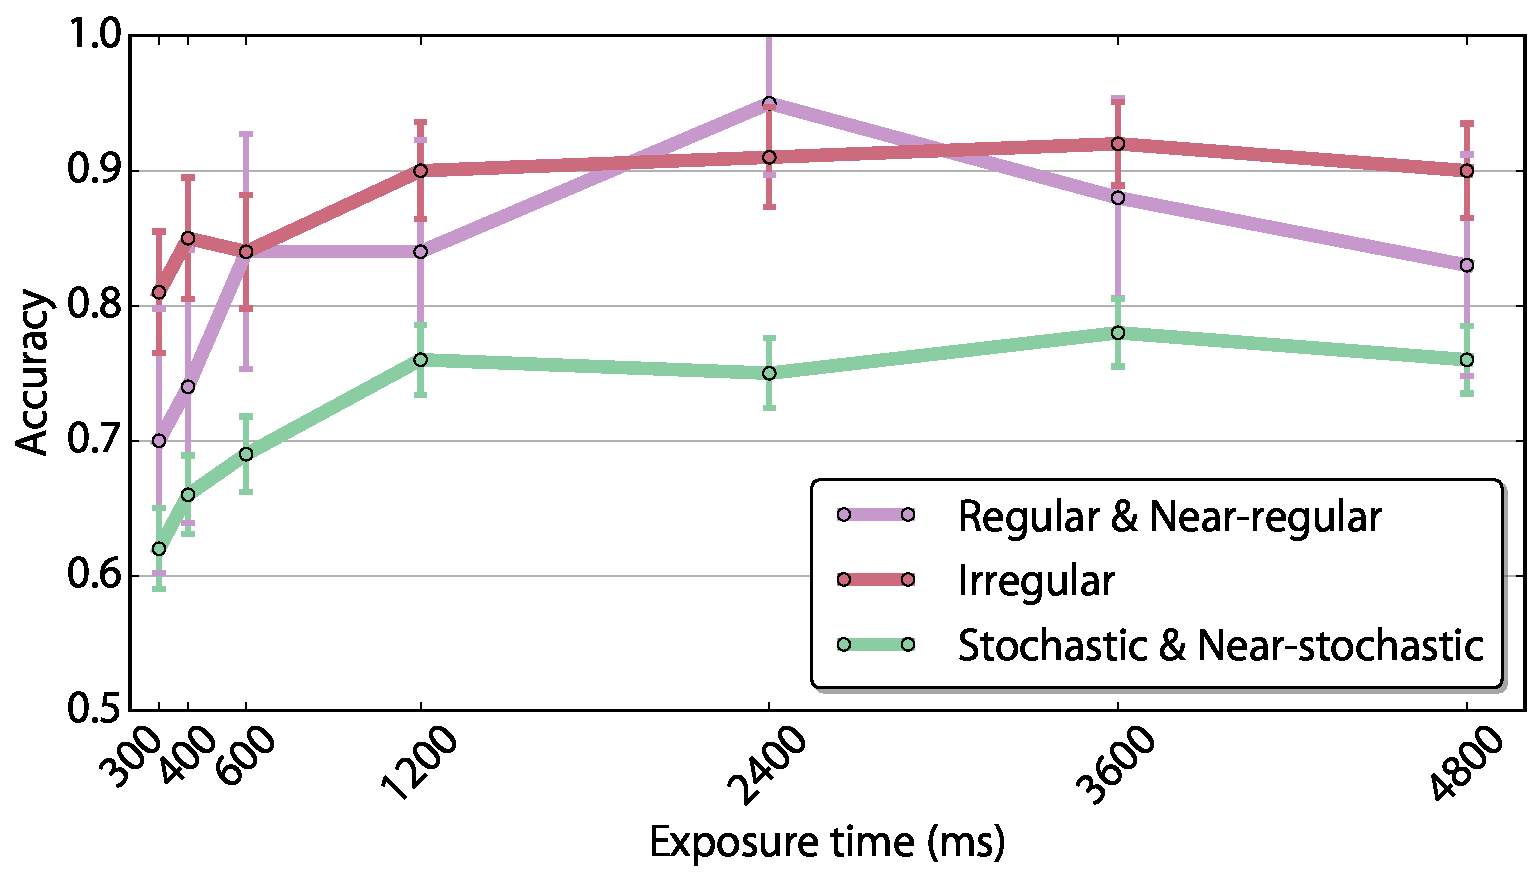
\epsfig{file=concat_appearance.pdf, width = 0.9\textwidth}\\
    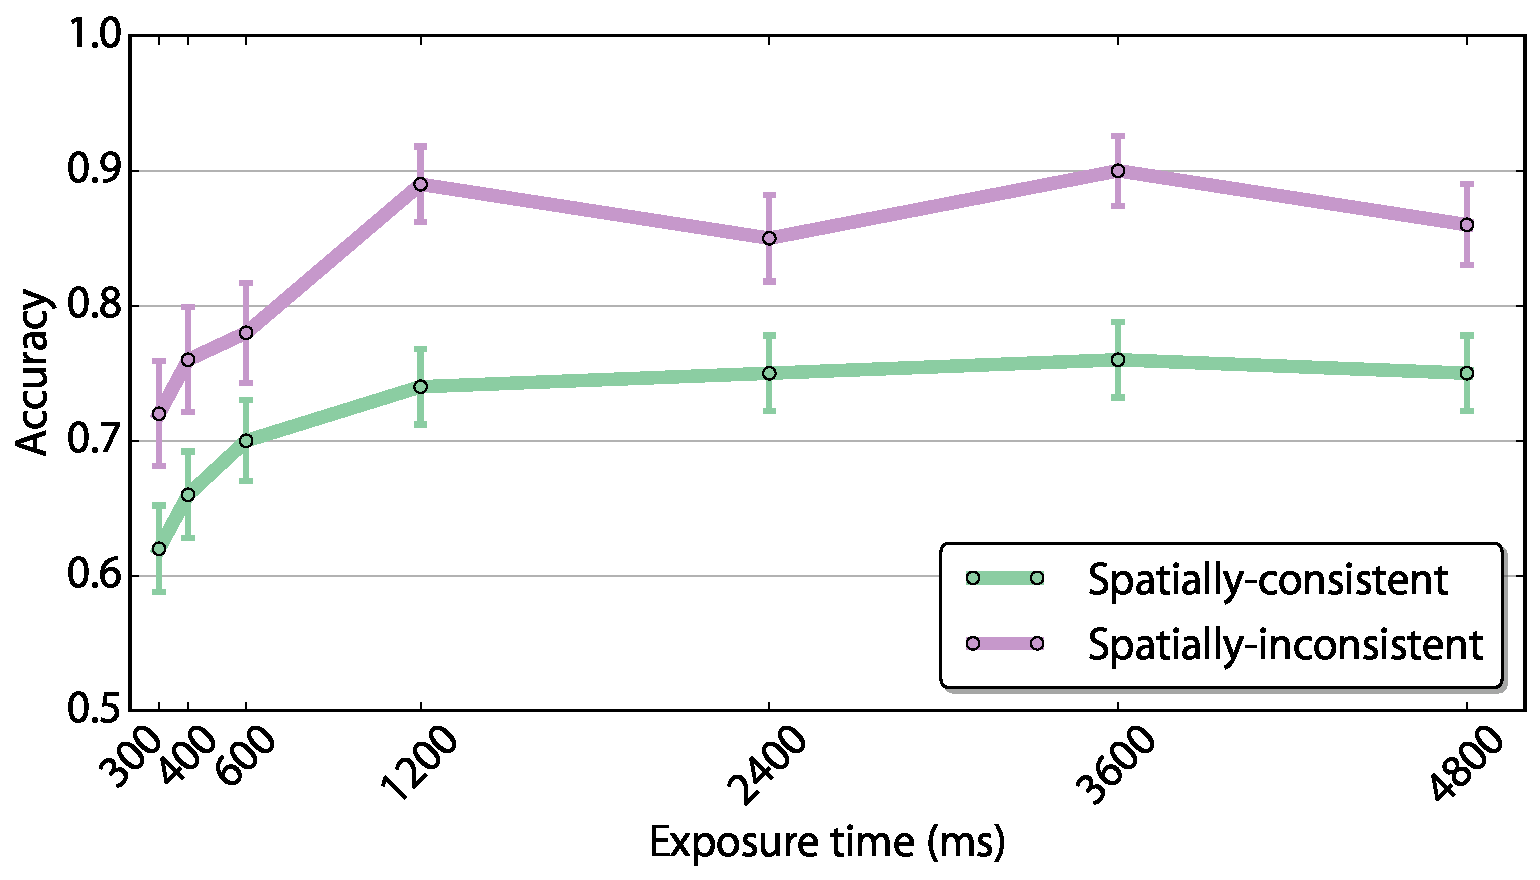
\epsfig{file=concat_dynamics.pdf, width = 0.9\textwidth}
	\caption[Time-limited pairwise comparisons across all textures, grouped by appearance and dynamics.]{Time-limited pairwise comparisons across all textures, grouped by appearance (top) and dynamics (bottom).  Shown with $95\%$ statistical confidence intervals.
	}
	\label{fig:pairwise_grouped}
	\vspace{-0.2cm}
\end{figure}

A full breakdown of the user study results by dynamic texture and 
grouping can be found in Appendix \ref{sec:full_user_study_results}.
Here some of the overall trends are discussed.

\subsubsection{Appearance-based analysis}

Based on appearance it is clear that textures with
large-scale spatial consistencies (regular, near-regular, 
and irregular textures) tend to perform poorly.
Examples being \path{flag} and \path{fountain_2} with
user accuracies of $98.9\% \pm 1.6\%$ and $90.8\% \pm 4.3\%$ 
averaged across all exposures, respectively.
This result is not unexpected and is a fundamental limitation of the 
local nature of the Gram matrix representation used in the 
appearance stream which was observed in static texture synthesis 
\cite{gatys2015}.
In contrast, stochastic and near-stochastic dynamic textures 
performed significantly better as their smaller-scale local 
variations are well captured by the appearance stream, for 
instance \path{water_1} and \path{lava} which had 
average accuracies of $53.8\% \pm 7.4\%$ and
$55.6\% \pm 7.4\%$, respectively, making them both 
statistically indistinguishable from real.

\subsubsection{Dynamics-based analysis}

In terms of dynamics, the user study showed that textures with
spatially-consistent dynamics (\eg, \path{tv_static}, 
\path{water_*}, and  \path{calm_water_*}) perform 
significantly better than those with spatially-inconsistent 
dynamics (\eg, \path{candle_flame}, \path{fountain_2}, 
and \path{snake_*}), where the dynamics drastically differ 
across spatial locations.
For example, \path{tv_static} and \path{calm_water_6}
have average accuracies of $48.6\% \pm 7.4\%$ and
$63.2\% \pm 7.2\%$, respectively, while
\path{candle_flame} and \path{snake_5} have average 
accuracies of $92.4\% \pm 4\%$ and $92.1\% \pm 4\%$, 
respectively.
Overall, the two-stream model is capable of reproducing a full spectrum
of spatially-consistent dynamics.
However, as the appearance shifts from containing small-scale 
spatial consistencies to containing large-scale spatial consistencies,
performance degrades.
This pattern was evident in the user study where the best-performing 
textures typically consisted of a stochastic or
near-stochastic appearance with spatially-consistent 
dynamics.
In contrast, the worst-performing textures consisted of
regular, near-regular, or irregular appearance with
spatially-inconsistent dynamics.

\section{Qualitative comparisons}

In this section, a qualitative comparison with the extant methods of Funke 
\etal \cite{funke2017} and Xie \etal \cite{xie2017synthesizing} is performed.
Generally, results from the proposed two-stream model are found to be qualitatively comparable or better than these methods.

To note, Funke \etal provided results on
only five textures and of those only four
are dynamic textures in the sense that their appearance
and dynamics are spatiotemporally coherent.
Their results on these sequences (\path{cranberries}, \path{flames}, 
\path{leaves}, and \path{water_5}) are included in the folder
\path{funke} under \path{dynamic_texture_synthesis/comparisons} in the supplementary material. The results from the two-stream model are included as well. An example on the \path{leaves} sequence is shown in Fig.\ \ref{fig:funke_comparison}.

\begin{figure}[t]
\begin{center}
\begin{tabular}{ >{\centering\arraybackslash} m{0.16\textwidth} || >{\centering\arraybackslash} m{0.80\textwidth} }
{target (\path{leaves})} & 
\showtexture{leaves/frame_} \\
\hline \hline
{Funke \etal \cite{funke2017}} &
\showtexture{leaves_funke/frame_} \\
\hline
{two-stream model} & 
\showtexture{leaves_output/frame_} \\
\end{tabular}
\end{center}
\vspace{-0.45cm}
\caption[Qualitative comparison with Funke \etal's \cite{funke2017} model]{Qualitative comparison with Funke \etal's \cite{funke2017} model on one of the sequences used in their work. Note that this sequence does not follow the thesis' assumption of a dynamic texture\highlight{, in the sense that the appearance and/or dynamics are not spatiotemporally homogeneous}.
(top row) Target sequence.
(middle row)
Dynamic texture synthesis when using Funke \etal's model. The model fails to capture the up-right motion of the leaves.
(bottom row)
Dynamic texture synthesis when using the proposed two-stream model. The up-right motion of the leaves is captured. Results are best viewed in video.
}
\label{fig:funke_comparison}
\end{figure}



Results are also compared on nine dynamic textures chosen to cover the full
range of the dynamics and appearance groupings introduced in the user study.
Publicly available code from Funke \etal and Xie \etal is used to produce their
results with their default parameter settings. For
Funke \etal's model, the parameters used are $\Delta{t}=4$ and
$T=12$ (recall that target dynamic textures
consist of 12 frames). For the spatiotemporal and temporal models from Xie
\etal, the parameters used are $T=1200$ and
$\tilde{M}=3$.
A comparison between the results from the proposed two-stream model, Funke
\etal's model, and Xie \etal's model
on the nine dynamic textures are included in the folder \path{xie_and_funke}
under \path{dynamic_texture_synthesis/comparisons}. An example on the \path{smoke_plume_1} dynamic texture is shown in Fig.\ \ref{fig:funke_xie_comparison}.

Note for Xie \etal, comparisons are made with their
spatiotemporal model, labelled ``Xie et al.\ (ST)'', designed for dynamic
textures with both spatial and temporal homogeneity, and their temporal model,
labelled ``Xie et al.\ (FC)'', designed for dynamic textures with only temporal
homogeneity.

\clearpage
\begin{figure}[t]
\begin{center}
\begin{tabular}{ >{\centering\arraybackslash} m{0.16\textwidth} || >{\centering\arraybackslash} m{0.80\textwidth} }
{target \break(\footnotesize\path{smoke_plume_1})} & 
\showtexture{smoke_plume_1/frame_} \\
\hline \hline
{Funke \etal \cite{funke2017}} &
\showtexture{smoke_plume_1_funke/frame_} \\
\hline
{Xie \etal \cite{xie2017synthesizing} (ST)} & 
\showtexture{smoke_plume_1_xie_st/frame_} \\
\hline
{Xie \etal \cite{xie2017synthesizing} (FC)} & 
\showtexture{smoke_plume_1_xie_fc/frame_} \\
\hline
{two-stream model} & 
\showtexture{smoke_plume_1_output/frame_} \\
\end{tabular}
\end{center}
\vspace{-0.45cm}
\caption[Qualitative comparison with Funke \etal's \cite{funke2017} and Xie \etal's \cite{xie2017synthesizing} model]{Qualitative comparison with Funke \etal's \cite{funke2017} and Xie \etal's \cite{xie2017synthesizing} models on one of the dynamic textures collected in this thesis.
(top row) Target dynamic texture.
(second row)
Dynamic texture synthesis when using Funke \etal's model.
(third row)
Dynamic texture synthesis when using Xie \etal's spatiotemporal model.
(fourth row)
Dynamic texture synthesis when using Xie \etal's temporal model.
(bottom row)
Dynamic texture synthesis when using the proposed two-stream model.
}
\label{fig:funke_xie_comparison}
\end{figure}


\clearpage

Overall, the results from the proposed two-stream model appear
qualitatively better, showing more temporal coherence and similarity
in dynamics as well as fewer spatial and temporal artifacts, such as blur and flicker, respectively.
This may be a natural consequence of the limited representation of dynamics
in both Funke \etal's and Xie \etal's models. Although the spatiotemporal model
of Xie \etal \cite{xie2017synthesizing} is able to synthesize dynamic textures
that lack spatial homogeneity (\eg, \path{bamboo} and \path{escalator}),
note that their method appears to not be able to synthesize novel dynamic textures, \ie, it
appears to faithfully reproduce the target texture, reducing the generalizability (\eg, synthesis of textures beyond the spatiotemporal extent of the input) of their approach, and thus its applicability.
 
As a consequence of jointly modelling appearance and dynamics, both methods \cite{funke2017,xie2017synthesizing} are not capable of the novel form of style
transfer that was demonstrated above. This capability was enabled by the factored
representation of dynamics and appearance. Furthermore, the spatiotemporal
extent of the output sequence generated by Xie \etal's
\cite{xie2017synthesizing} method is limited to being equal to the input.
The proposed approach does not share this limitation.

\section{Discussion}

This chapter provided a qualitative analysis on a variety of results obtained using the proposed two-stream model for dynamic texture synthesis, incremental texture synthesis, temporally-endless texture synthesis, and dynamics style transfer. For dynamic texture synthesis, it was shown that both the appearance and dynamics streams were required to synthesize dynamic textures that matched both the framewise appearance of the target and its dynamics. For incremental texture synthesis, it was shown that incrementally synthesized dynamic textures exhibited no divergence or degradation when compared to those synthesized using the typical batch process. For temporally-endless texture synthesis, it was shown that the synthesized dynamic textures exhibited no apparent temporal discontinuity between the last and first frames. For dynamics style transfer, it was shown that the dynamics of one dynamic texture can be successfully combined with the appearance of another, under the stipulation that the appearance and dynamics targets came from textures similar in scale and semantics.

Additionally, a large-scale user study was performed to quantitatively evaluate the realism of dynamic textures synthesized by the proposed model by comparing synthesized results with their respective targets. An evaluation on a baseline version of the model was performed as well. Overall, dynamic textures synthesized by the two-stream model were able to fool users $33.9\% \pm 2.5\%$ of the time for brief exposures. In contrast, dynamic textures synthesized by the baseline model were able to fool users $10.2\% \pm 1.8\%$ of the time. 
Although the final two-stream model was statistically better than the baseline model, users were still able to reliably tell the difference between real and synthesized for longer exposure times. Specifically, $79.6\% \pm 1.1\%$ of the time, they could distinguish real from synthesized when exposure times were 1.2 seconds or higher. It is possible that for longer exposure times, spatial artifacts (\eg, chromatic aberration and noise) of the synthesized texture may have served as cues for distinguishing between real and synthesized. These artifacts suggest room for improvement on the representation of appearance and has been left for future work.

Finally, a qualitative comparison with two extant methods for dynamic texture synthesis was performed. Overall, the results from the proposed two-stream model were shown to be qualitatively better than the compared methods, showing more temporal coherence and similarity in dynamics as well as fewer spatial and temporal artifacts. Furthermore, it is unclear how the other methods can be applied to the novel dynamics style transfer, as can the proposed two-stream model.

\chapter{Conclusion \todomatthew{haven't touched yet}}
In this paper, we presented a novel, two-stream model
of dynamic textures using ConvNets to represent the appearance and
dynamics.
We applied this model to a variety of dynamic texture synthesis
tasks and showed that, so long as the input textures are generally
true dynamic textures, \ie, have spatially invariant statistics and
spatiotemporally invariant dynamics, the resulting synthesized 
textures are compelling.
This was validated both qualitatively and quantitatively through
a large user study.
Further, we showed that the two-stream model enabled dynamics
style transfer, where the appearance and dynamics 
information from different sources can be combined to generate
a novel texture.

We have explored this model thoroughly and found a few limitations which we leave as directions for future work.
First, much like has been reported in recent image style transfer
work \cite{gatys2016image}, we have found that high frequency
noise and chromatic aberrations are a problem in generation.
Another issue that arises is the model fails to capture
textures with spatially-variant appearance, (\eg, 
\texttt{flag} in Fig.\ \ref{fig:failures}) and
spatially-inconsistent dynamics (\eg, \texttt{escalator} in 
Fig.\ \ref{fig:failures}).
By collapsing the local statistics into a Gram matrix, 
the spatial and temporal organization is lost.
Simple post-processing methods may alleviate some of these issues
but we believe that they also point to a need for a better
representation.
Beyond addressing these limitations, a natural next step would be
to extend the idea of a factorized representation into feed-forward
generative networks that have found success in static image
synthesis, \eg, \cite{johnson2016,ulyanov2016}.

\bibliographystyle{plain}
\bibliography{thesis-short,thesis}
%\todos

%------------Appendix--------------%
\myappendix{Appendix}

\section{Experimental procedure}\label{sec:experimental_procedure}
Provided here are the experimental details of the user study
using Amazon Mechanical Turk (AMT). Experimental trials were
grouped into batches of Human Intelligence Tasks (HITs) for
users to complete. Each HIT consisted of 59 pairwise
comparisons between a synthesized dynamic texture and its target.
Users were asked to choose which texture appeared more realistic
after viewing each texture independently for an exposure time (in seconds) 
sampled randomly from the set \{0.3, 0.4, 0.6, 1.2, 2.4, 3.6, 4.8\}.
Note that 12 frames of the dynamic texture corresponds to 1.2 seconds, \ie, 10 frames per second. Since the dynamic textures were collected from various sources with varying framerates, a canonical framerate was chosen for all input and synthesized dynamic textures. 10 frames per second was chosen to allow sufficient viewing time (1.2 seconds) while maintaining easily distinguishable dynamics.
Before viewing a dynamic texture, a centred dot is flashed twice to
indicate to the user where to look (left or right).
To prepare users for the task, the first three comparisons 
were used for warm-up, exposing them to the shortest (0.3s), 
median (1.2s), and longest (4.8s) durations.
To prevent spamming and bias, the experiment was constrained as 
follows:
\begin{enumerate}
	\item Users could make a choice only after both dynamic textures were shown;
	\item The next texture comparison could only be made after a decision was made for the current comparison;
	\item A choice could not be changed after the next pair of dynamic textures were shown;
	\item Users were each restricted to a single HIT.
\end{enumerate}
Obvious unrealistic dynamic textures were synthesized by 
terminating synthesis early (100 iterations) and were used as sentinel tests. An example is shown in Fig.\ \ref{fig:sentinel}.

\begin{figure}[t]
\begin{center}
\begin{tabular}{ >{\centering\arraybackslash} m{0.16\textwidth} || >{\centering\arraybackslash} m{0.80\textwidth} }
{target (\path{water_1})} & 
\showtexture{water_1/frame_} \\
\hline \hline
{synthesized} &
\showtexture{water_1_output/frame_} \\
\hline
{sentinel} & 
\showtexture{water_1_sentinel/frame_} \\
\end{tabular}
\end{center}
\vspace{-0.45cm}
\caption[Example of a sentinel dynamic texture for the user study]{Example of a sentinel dynamic texture for the user study.
(top row) Target dynamic texture.
(middle row)
An obviously-unrealistic synthesized dynamic texture (a sentinel example). Achieved by terminating synthesis early (100 optimization iterations).
(bottom row)
Dynamic texture synthesized after $6,000$ optimization iterations.
}
\label{fig:sentinel}
\end{figure}

Three of the 59 pairwise comparisons were sentinels and results from
users who gave incorrect answers on any of the sentinel
comparisons were not used. The left-right order of textures within a pair,
display order within a pair, and order of pairs within a HIT, were randomized.
An example of a HIT is shown in a video included with the supplemental material: \path{HIT_example.mp4}.

Users were paid \$2 USD per HIT, and were required to have at least
a 98\% HIT approval rating, greater than or equal to 5000 HITs
approved, and to be residing in the US. Results were collected from 200 unique 
users to evaluate the final model (which uses the ``Concat layer'') and another 200 to evaluate the baseline model (which uses the ``Flow decode layer'').

\section{Qualitative results}
Provided in the supplemental material are videos showcasing the qualitative results of the two-stream model, including the experiments mentioned in the main manuscript. The videos are in MP4 format (H.264 codec) and are best viewed in a loop. They are enclosed in the following folders:
\begin{itemize}
	\item \path{target_textures}: This folder contains the 59 dynamic textures used as targets for synthesis.
	\item \path{dynamic_texture_synthesis}: This folder contains synthesized dynamic textures where the appearance and dynamics targets are the same.
	\item \path{using_concatenation_layer}: This folder contains synthesized dynamic textures where the concatenation layer was used for computing the Gramian on the dynamics stream. These are the results from the final model.
	\item \path{using_flow_decode_layer}: This folder contains synthesized dynamic textures where the predicted flow output is used for computing the Gramian on the dynamics stream. These are the results from the baseline.
	\item \path{full_synthesis}: This folder contains regularly-synthesized dynamic textures, \ie, not incrementally-generated, nor temporally-endless, etc.
	\item \path{appearance_stream_only}: This folder contains dynamic textures synthesized using only the appearance stream of the two-stream model. The dynamics stream is not used.
	\item \path{incrementally_generated}: This folder contains dynamic textures synthesized using the incremental process outlined in Sec.\ \ref{sec:incremental_synthesis} in the main manuscript.
	\item \path{temporally_endless}: This folder contains a synthesized dynamic texture (\path{smoke_plume_1}) where there is no discernible temporal seam between the last and first frames. Played as a loop, it appears to be temporally endless, thus, it is presented in animated GIF format.
	\item \path{dynamics_style_transfer}: This folder contains synthesized dynamic textures where the appearance and dynamics targets are different. Also included are videos where the synthesized dynamic texture is ``pasted'' back onto the original image it was cropped from, showing a proof-of-concept of dynamics style transfer as an artistic tool.
	\item \path{comparisons/funke}: This folder contains four dynamic texture synthesis comparisons between the two-stream model and a recent (unpublished) approach \cite{funke2017}. The dynamic textures chosen are those reported by Funke \etal \cite{funke2017} which exhibit spatiotemporal homogeneity. For ease of comparison, the results from both models have been concatenated with their corresponding targets.
	\item \path{comparisons/xie_and_funke}: This folder contains nine dynamic texture synthesis comparisons between the two-stream model, Funke \etal's \cite{funke2017}, and Xie \etal's \cite{xie2017synthesizing}. The dynamic textures chosen cover the full range of the appearance and dynamics groupings listed in Sec.\ \ref{sec:user_study}. For ease of comparison, the results from all models have been concatenated with their corresponding targets.
\end{itemize}

\section{Full user study results}
Figures \ref{fig:alltextures_hist_short} and \ref{fig:alltextures_hist_long}
show histograms of the average user accuracy on each texture, averaged over a 
range of exposure times. The histogram bars are ordered from lowest
to highest accuracy, based on the results when using the final model.

Tables \ref{tab:table_concat} and \ref{tab:table_concat_range} show
the average user accuracy on each texture when using the final model.
The results are averaged over exposure times. Similarly, Tables
\ref{tab:table_flowdecode} and \ref{tab:table_flowdecode_range} show the results
when using the baseline.

Tables \ref{tab:table_concat_app} and \ref{tab:table_concat_app_range} show
the average user accuracy on texture appearance groups when using the
final model. The results are averaged over exposure times. Similarly, Tables
\ref{tab:table_flowdecode_app} and \ref{tab:table_flowdecode_app_range} show the results when using the baseline.

Tables \ref{tab:table_concat_dyn} and \ref{tab:table_concat_dyn_range} show
the average user accuracy on texture dynamics groups when using the
final model. The results are averaged over exposure times. Similarly, Tables
\ref{tab:table_flowdecode_dyn} and \ref{tab:table_flowdecode_dyn_range} show the results when using the baseline.

Tables \ref{tab:table_concat_all} and \ref{tab:table_concat_all_range} show
the average user accuracy over all textures when using the
final model. The results are averaged over exposure times. Similarly, Tables
\ref{tab:table_flowdecode_all} and \ref{tab:table_flowdecode_all_range} show the results when using the baseline.

\begin{sidewaysfigure*}[t]
	\centering
	\begin{subfigure}[b]{\textwidth}
		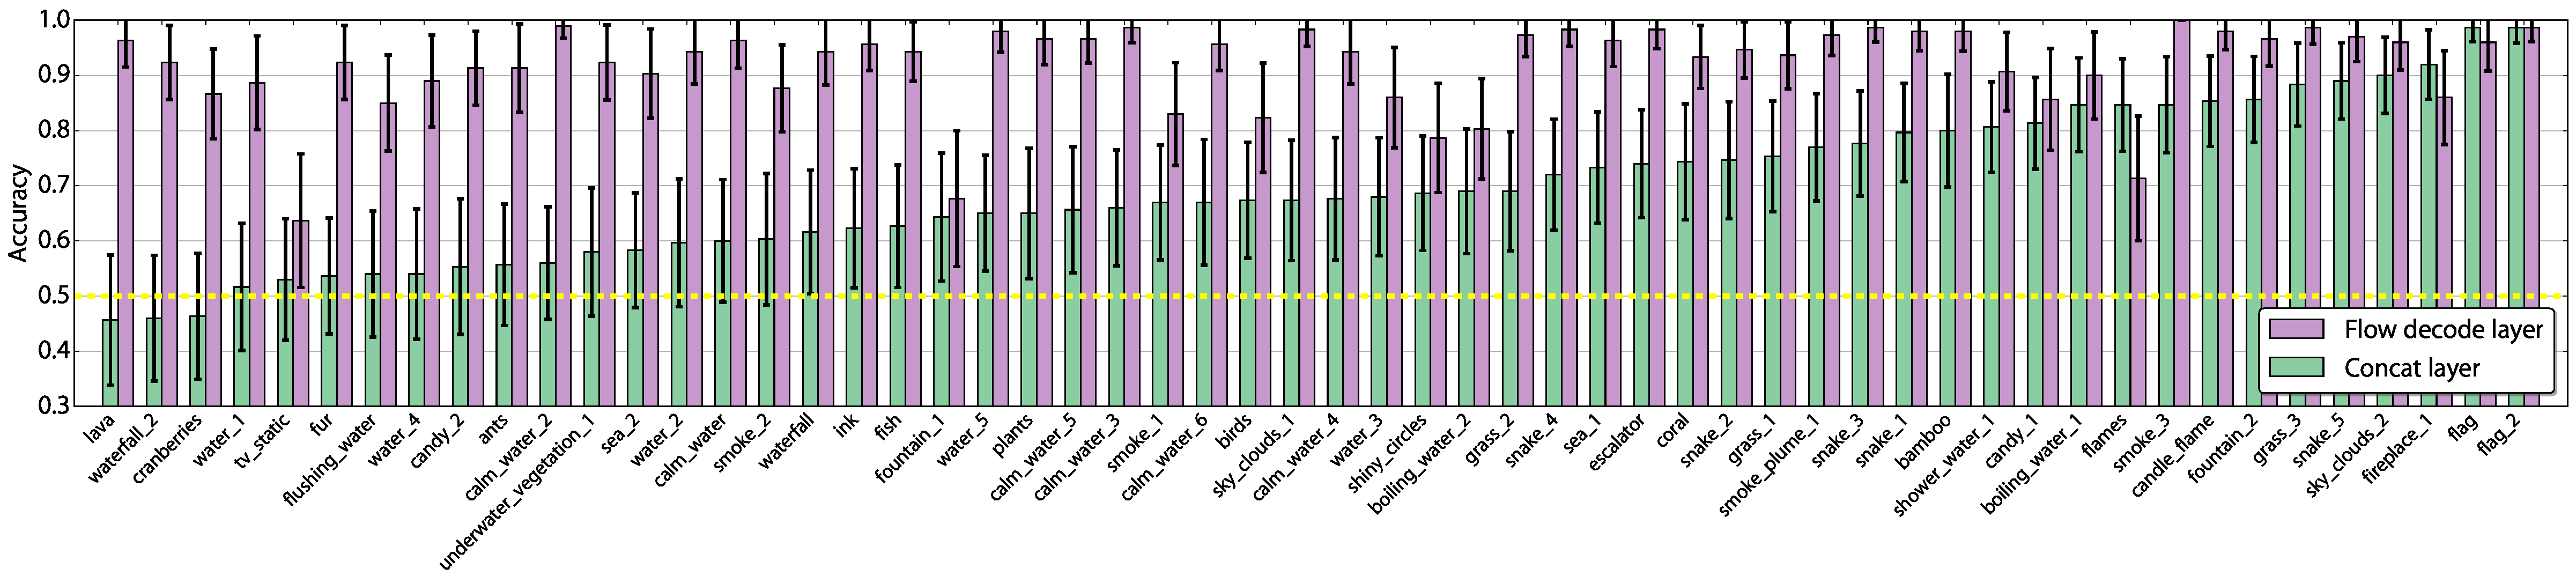
\epsfig{file=histogram_shortexposures.pdf, width = \textwidth}
		\vspace{-0.8cm}
		\caption{Short exposure times (300-600 ms).}
		\label{fig:alltextures_hist_short}
	\end{subfigure}
	\begin{subfigure}[b]{\textwidth}	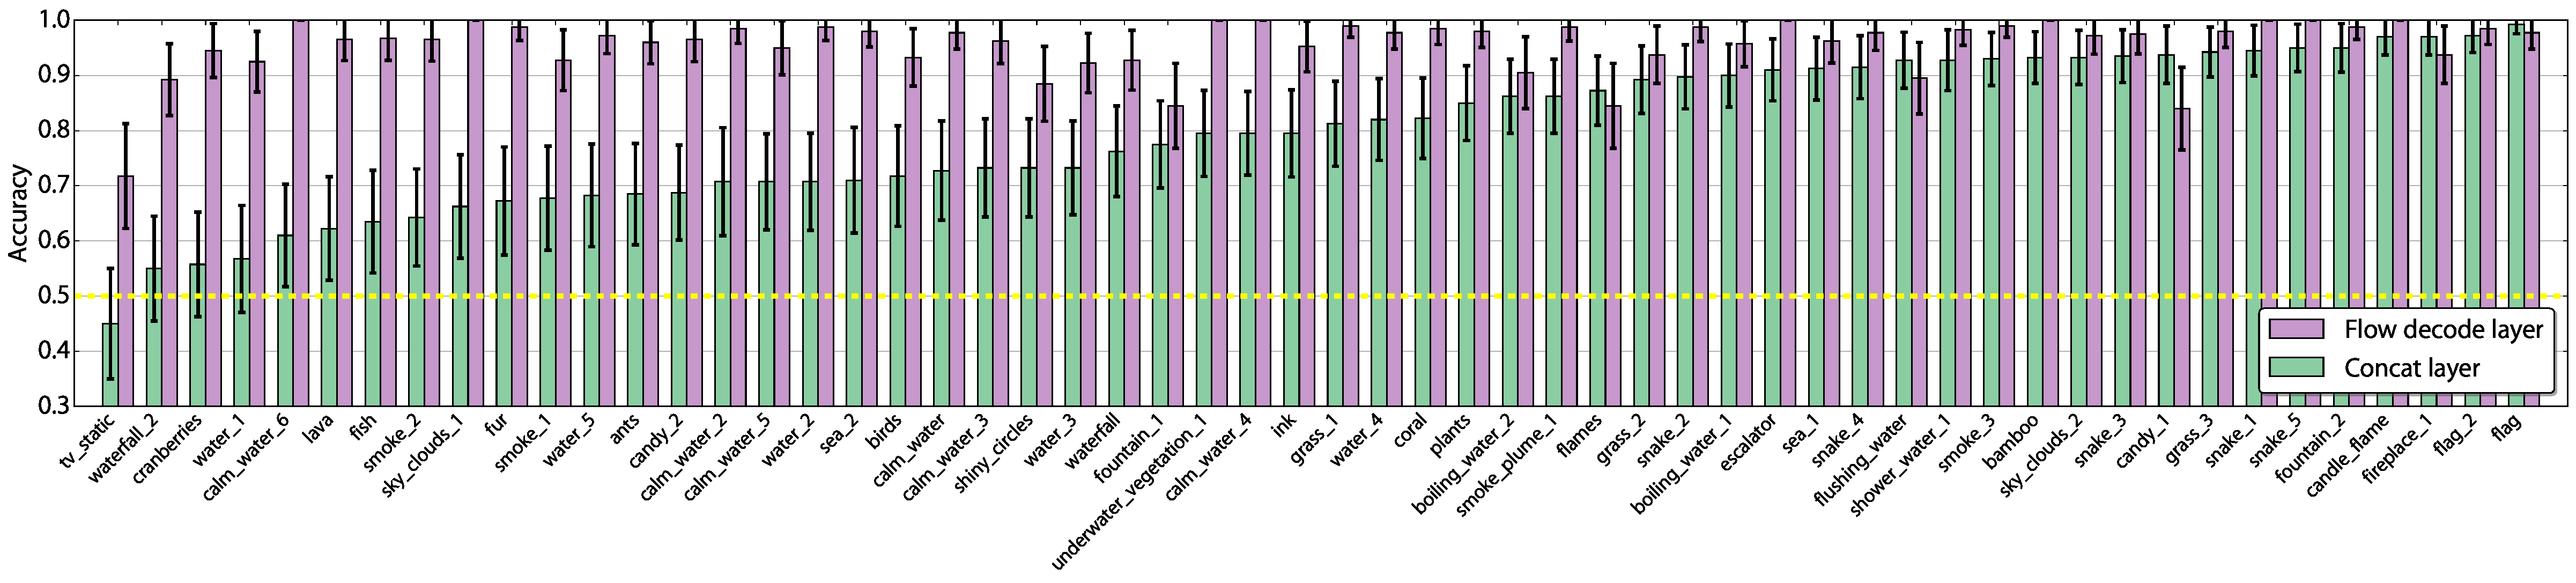
\epsfig{file=histogram_longexposures.pdf, width = \textwidth}
		\vspace{-0.55cm}
		\caption{Long exposure times (1200-4800 ms).}
		\label{fig:alltextures_hist_long}
	\end{subfigure}
	\vspace{-0.65cm}
	\caption[Per-texture accuracies averaged over exposure times]{Per-texture accuracies averaged over exposure times. Each texture accuracy includes a margin of error with a $95\%$ statistical confidence.}
	\vspace{-0.45cm}
	\label{fig:pertexture_hist}
\end{sidewaysfigure*}

\clearpage
\onecolumn
\begin{table*}
\centering
	\resizebox{0.9\textwidth}{!}{%
	\csvreader[tabular=|l|l|,
	    table head=\hline Dynamic texture & 300 ms.\\\hline\hline,
	    late after line=\\\hline]%
	{tables/all_textures_concat_300.csv}{Name=\Name,Accuracy=\Accuracy}%
	{\Name & \Accuracy}%
	\csvreader[tabular=|l|,
	    table head=\hline 400 ms.\\\hline\hline,
	    late after line=\\\hline]%
	{tables/all_textures_concat_400.csv}{Accuracy=\Accuracy}%
	{\Accuracy}%
	\csvreader[tabular=|l|,
	    table head=\hline 600 ms.\\\hline\hline,
	    late after line=\\\hline]%
	{tables/all_textures_concat_600.csv}{Accuracy=\Accuracy}%
	{\Accuracy}%
	\csvreader[tabular=|l|,
	    table head=\hline 1200 ms.\\\hline\hline,
	    late after line=\\\hline]%
	{tables/all_textures_concat_1200.csv}{Accuracy=\Accuracy}%
	{\Accuracy}%
	\csvreader[tabular=|l|,
	    table head=\hline 2400 ms.\\\hline\hline,
	    late after line=\\\hline]%
	{tables/all_textures_concat_2400.csv}{Accuracy=\Accuracy}%
	{\Accuracy}%
	\csvreader[tabular=|l|,
	    table head=\hline 3600 ms.\\\hline\hline,
	    late after line=\\\hline]%
	{tables/all_textures_concat_3600.csv}{Accuracy=\Accuracy}%
	{\Accuracy}%
	\csvreader[tabular=|l|,
	    table head=\hline 4800 ms.\\\hline\hline,
	    late after line=\\\hline]%
	{tables/all_textures_concat_4800.csv}{Accuracy=\Accuracy}%
	{\Accuracy}%
	}
	\caption[Per-texture accuracies averaged over exposure times, using the concatenation layer]{Per-texture accuracies averaged over exposure times, using the concatenation layer. Each texture accuracy includes a margin of error with a $95\%$ statistical confidence.}
	\label{tab:table_concat}
\end{table*}

\begin{table*}
	\centering
	\resizebox{0.65\textwidth}{!}{%
	\csvreader[tabular=|l|l|,
	    table head=\hline Dynamic texture & Short (300-600 ms.)\\\hline\hline,
	    late after line=\\\hline]%
	{tables/all_textures_concat_short.csv}{Name=\Name,Accuracy=\Accuracy}%
	{\Name & \Accuracy}%
	\csvreader[tabular=|l|,
	    table head=\hline Long (1200-4800 ms.)\\\hline\hline,
	    late after line=\\\hline]%
	{tables/all_textures_concat_long.csv}{Accuracy=\Accuracy}%
	{\Accuracy}%
	\csvreader[tabular=|l|,
	    table head=\hline All (300-4800 ms.)\\\hline\hline,
	    late after line=\\\hline]%
	{tables/all_textures_concat_all.csv}{Accuracy=\Accuracy}%
	{\Accuracy}%
	}
	\caption[Per-texture accuracies averaged over a range of exposure times, using the concatenation layer]{Per-texture accuracies averaged over a range of exposure times, using the concatenation layer. Each texture accuracy includes a margin of error with a $95\%$ statistical confidence.}
	\label{tab:table_concat_range}
\end{table*}

%%%%%%

\begin{table*}
	\centering
	\resizebox{0.9\textwidth}{!}{%
	\csvreader[tabular=|l|l|,
	    table head=\hline Dynamic texture & 300 ms.\\\hline\hline,
	    late after line=\\\hline]%
	{tables/all_textures_flowdecode_300.csv}{Name=\Name,Accuracy=\Accuracy}%
	{\Name & \Accuracy}%
	\csvreader[tabular=|l|,
	    table head=\hline 400 ms.\\\hline\hline,
	    late after line=\\\hline]%
	{tables/all_textures_flowdecode_400.csv}{Accuracy=\Accuracy}%
	{\Accuracy}%
	\csvreader[tabular=|l|,
	    table head=\hline 600 ms.\\\hline\hline,
	    late after line=\\\hline]%
	{tables/all_textures_flowdecode_600.csv}{Accuracy=\Accuracy}%
	{\Accuracy}%
	\csvreader[tabular=|l|,
	    table head=\hline 1200 ms.\\\hline\hline,
	    late after line=\\\hline]%
	{tables/all_textures_flowdecode_1200.csv}{Accuracy=\Accuracy}%
	{\Accuracy}%
	\csvreader[tabular=|l|,
	    table head=\hline 2400 ms.\\\hline\hline,
	    late after line=\\\hline]%
	{tables/all_textures_flowdecode_2400.csv}{Accuracy=\Accuracy}%
	{\Accuracy}%
	\csvreader[tabular=|l|,
	    table head=\hline 3600 ms.\\\hline\hline,
	    late after line=\\\hline]%
	{tables/all_textures_flowdecode_3600.csv}{Accuracy=\Accuracy}%
	{\Accuracy}%
	\csvreader[tabular=|l|,
	    table head=\hline 4800 ms.\\\hline\hline,
	    late after line=\\\hline]%
	{tables/all_textures_flowdecode_4800.csv}{Accuracy=\Accuracy}%
	{\Accuracy}%
	}
	\caption[Per-texture accuracies averaged over exposure times, using the flow decode layer]{Per-texture accuracies averaged over exposure times, using the flow decode layer. Each texture accuracy includes a margin of error with a $95\%$ statistical confidence.}
	\label{tab:table_flowdecode}
\end{table*}

\begin{table*}
	\centering
	\resizebox{0.65\textwidth}{!}{%
	\csvreader[tabular=|l|l|,
	    table head=\hline Dynamic texture & Short (300-600 ms.)\\\hline\hline,
	    late after line=\\\hline]%
	{tables/all_textures_flowdecode_short.csv}{Name=\Name,Accuracy=\Accuracy}%
	{\Name & \Accuracy}%
	\csvreader[tabular=|l|,
	    table head=\hline Long (1200-4800 ms.)\\\hline\hline,
	    late after line=\\\hline]%
	{tables/all_textures_flowdecode_long.csv}{Accuracy=\Accuracy}%
	{\Accuracy}%
	\csvreader[tabular=|l|,
	    table head=\hline All (300-4800 ms.)\\\hline\hline,
	    late after line=\\\hline]%
	{tables/all_textures_flowdecode_all.csv}{Accuracy=\Accuracy}%
	{\Accuracy}%
	}
	\caption[Per-texture accuracies averaged over a range of exposure times, using the flow decode layer]{Per-texture accuracies averaged over a range of exposure times, using the flow decode layer. Each texture accuracy includes a margin of error with a $95\%$ statistical confidence.}
	\label{tab:table_flowdecode_range}
\end{table*}

%%%%%%

\clearpage
\begin{table*}
	\centering
	\resizebox{0.9\textwidth}{!}{%
	\csvreader[tabular=|l|l|,
	    table head=\hline Appearance group & 300 ms.\\\hline\hline,
	    late after line=\\\hline]%
	{tables/appearance_grouping_concat_300.csv}{Name=\Name,Accuracy=\Accuracy}%
	{\Name & \Accuracy}%
	\csvreader[tabular=|l|,
	    table head=\hline 400 ms.\\\hline\hline,
	    late after line=\\\hline]%
	{tables/appearance_grouping_concat_400.csv}{Accuracy=\Accuracy}%
	{\Accuracy}%
	\csvreader[tabular=|l|,
	    table head=\hline 600 ms.\\\hline\hline,
	    late after line=\\\hline]%
	{tables/appearance_grouping_concat_600.csv}{Accuracy=\Accuracy}%
	{\Accuracy}%
	\csvreader[tabular=|l|,
	    table head=\hline 1200 ms.\\\hline\hline,
	    late after line=\\\hline]%
	{tables/appearance_grouping_concat_1200.csv}{Accuracy=\Accuracy}%
	{\Accuracy}%
	\csvreader[tabular=|l|,
	    table head=\hline 2400 ms.\\\hline\hline,
	    late after line=\\\hline]%
	{tables/appearance_grouping_concat_2400.csv}{Accuracy=\Accuracy}%
	{\Accuracy}%
	\csvreader[tabular=|l|,
	    table head=\hline 3600 ms.\\\hline\hline,
	    late after line=\\\hline]%
	{tables/appearance_grouping_concat_3600.csv}{Accuracy=\Accuracy}%
	{\Accuracy}%
	\csvreader[tabular=|l|,
	    table head=\hline 4800 ms.\\\hline\hline,
	    late after line=\\\hline]%
	{tables/appearance_grouping_concat_4800.csv}{Accuracy=\Accuracy}%
	{\Accuracy}%
	}
	\caption[Accuracies of textures grouped by appearances, averaged over exposure times, using the concatenation layer]{Accuracies of textures grouped by appearances, averaged over exposure times, using the concatenation layer. Each texture accuracy includes a margin of error with a $95\%$ statistical confidence.}
	\label{tab:table_concat_app}
\end{table*}

\begin{table*}
	\centering
	\resizebox{0.65\textwidth}{!}{%
	\csvreader[tabular=|l|l|,
	    table head=\hline Appearance group & Short (300-600 ms.)\\\hline\hline,
	    late after line=\\\hline]%
	{tables/appearance_grouping_concat_short.csv}{Name=\Name,Accuracy=\Accuracy}%
	{\Name & \Accuracy}%
	\csvreader[tabular=|l|,
	    table head=\hline Long (1200-4800 ms.)\\\hline\hline,
	    late after line=\\\hline]%
	{tables/appearance_grouping_concat_long.csv}{Accuracy=\Accuracy}%
	{\Accuracy}%
	\csvreader[tabular=|l|,
	    table head=\hline All (300-4800 ms.)\\\hline\hline,
	    late after line=\\\hline]%
	{tables/appearance_grouping_concat_all.csv}{Accuracy=\Accuracy}%
	{\Accuracy}%
	}
	\caption[Accuracies of textures grouped by appearances, averaged over a range of exposure times, using the concatenation layer]{Accuracies of textures grouped by appearances, averaged over a range of exposure times, using the concatenation layer. Each texture accuracy includes a margin of error with a $95\%$ statistical confidence.}
	\label{tab:table_concat_app_range}
\end{table*}

\begin{table*}
	\centering
	\resizebox{0.9\textwidth}{!}{%
	\csvreader[tabular=|l|l|,
	    table head=\hline Appearance group & 300 ms.\\\hline\hline,
	    late after line=\\\hline]%
	{tables/appearance_grouping_flowdecode_300.csv}{Name=\Name,Accuracy=\Accuracy}%
	{\Name & \Accuracy}%
	\csvreader[tabular=|l|,
	    table head=\hline 400 ms.\\\hline\hline,
	    late after line=\\\hline]%
	{tables/appearance_grouping_flowdecode_400.csv}{Accuracy=\Accuracy}%
	{\Accuracy}%
	\csvreader[tabular=|l|,
	    table head=\hline 600 ms.\\\hline\hline,
	    late after line=\\\hline]%
	{tables/appearance_grouping_flowdecode_600.csv}{Accuracy=\Accuracy}%
	{\Accuracy}%
	\csvreader[tabular=|l|,
	    table head=\hline 1200 ms.\\\hline\hline,
	    late after line=\\\hline]%
	{tables/appearance_grouping_flowdecode_1200.csv}{Accuracy=\Accuracy}%
	{\Accuracy}%
	\csvreader[tabular=|l|,
	    table head=\hline 2400 ms.\\\hline\hline,
	    late after line=\\\hline]%
	{tables/appearance_grouping_flowdecode_2400.csv}{Accuracy=\Accuracy}%
	{\Accuracy}%
	\csvreader[tabular=|l|,
	    table head=\hline 3600 ms.\\\hline\hline,
	    late after line=\\\hline]%
	{tables/appearance_grouping_flowdecode_3600.csv}{Accuracy=\Accuracy}%
	{\Accuracy}%
	\csvreader[tabular=|l|,
	    table head=\hline 4800 ms.\\\hline\hline,
	    late after line=\\\hline]%
	{tables/appearance_grouping_flowdecode_4800.csv}{Accuracy=\Accuracy}%
	{\Accuracy}%
	}
	\caption[Accuracies of textures grouped by appearances, averaged over exposure times, using the flow decode layer]{Accuracies of textures grouped by appearances, averaged over exposure times, using the flow decode layer. Each texture accuracy includes a margin of error with a $95\%$ statistical confidence.}
	\label{tab:table_flowdecode_app}
\end{table*}

\begin{table*}
	\centering
	\resizebox{0.65\textwidth}{!}{%
	\csvreader[tabular=|l|l|,
	    table head=\hline Appearance group & Short (300-600 ms.)\\\hline\hline,
	    late after line=\\\hline]%
	{tables/appearance_grouping_flowdecode_short.csv}{Name=\Name,Accuracy=\Accuracy}%
	{\Name & \Accuracy}%
	\csvreader[tabular=|l|,
	    table head=\hline Long (1200-4800 ms.)\\\hline\hline,
	    late after line=\\\hline]%
	{tables/appearance_grouping_flowdecode_long.csv}{Accuracy=\Accuracy}%
	{\Accuracy}%
	\csvreader[tabular=|l|,
	    table head=\hline All (300-4800 ms.)\\\hline\hline,
	    late after line=\\\hline]%
	{tables/appearance_grouping_flowdecode_all.csv}{Accuracy=\Accuracy}%
	{\Accuracy}%
	}
	\caption[Accuracies of textures grouped by appearances, averaged over a range of exposure times, using the flow decode layer]{Accuracies of textures grouped by appearances, averaged over a range of exposure times, using the flow decode layer. Each texture accuracy includes a margin of error with a $95\%$ statistical confidence.}
	\label{tab:table_flowdecode_app_range}
\end{table*}
\clearpage

%%%%%%

\clearpage
\begin{table*}
	\centering
	\resizebox{0.9\textwidth}{!}{%
	\csvreader[tabular=|l|l|,
	    table head=\hline Dynamics group & 300 ms.\\\hline\hline,
	    late after line=\\\hline]%
	{tables/dynamics_grouping_concat_300.csv}{Name=\Name,Accuracy=\Accuracy}%
	{\Name & \Accuracy}%
	\csvreader[tabular=|l|,
	    table head=\hline 400 ms.\\\hline\hline,
	    late after line=\\\hline]%
	{tables/dynamics_grouping_concat_400.csv}{Accuracy=\Accuracy}%
	{\Accuracy}%
	\csvreader[tabular=|l|,
	    table head=\hline 600 ms.\\\hline\hline,
	    late after line=\\\hline]%
	{tables/dynamics_grouping_concat_600.csv}{Accuracy=\Accuracy}%
	{\Accuracy}%
	\csvreader[tabular=|l|,
	    table head=\hline 1200 ms.\\\hline\hline,
	    late after line=\\\hline]%
	{tables/dynamics_grouping_concat_1200.csv}{Accuracy=\Accuracy}%
	{\Accuracy}%
	\csvreader[tabular=|l|,
	    table head=\hline 2400 ms.\\\hline\hline,
	    late after line=\\\hline]%
	{tables/dynamics_grouping_concat_2400.csv}{Accuracy=\Accuracy}%
	{\Accuracy}%
	\csvreader[tabular=|l|,
	    table head=\hline 3600 ms.\\\hline\hline,
	    late after line=\\\hline]%
	{tables/dynamics_grouping_concat_3600.csv}{Accuracy=\Accuracy}%
	{\Accuracy}%
	\csvreader[tabular=|l|,
	    table head=\hline 4800 ms.\\\hline\hline,
	    late after line=\\\hline]%
	{tables/dynamics_grouping_concat_4800.csv}{Accuracy=\Accuracy}%
	{\Accuracy}%
	}
	\caption[Accuracies of textures grouped by dynamics, averaged over exposure times, using the concatenation layer]{Accuracies of textures grouped by dynamics, averaged over exposure times, using the concatenation layer. Each texture accuracy includes a margin of error with a $95\%$ statistical confidence.}
	\label{tab:table_concat_dyn}
\end{table*}

\begin{table*}
	\centering
	\resizebox{0.65\textwidth}{!}{%
	\csvreader[tabular=|l|l|,
	    table head=\hline Dynamics group & Short (300-600 ms.)\\\hline\hline,
	    late after line=\\\hline]%
	{tables/dynamics_grouping_concat_short.csv}{Name=\Name,Accuracy=\Accuracy}%
	{\Name & \Accuracy}%
	\csvreader[tabular=|l|,
	    table head=\hline Long (1200-4800 ms.)\\\hline\hline,
	    late after line=\\\hline]%
	{tables/dynamics_grouping_concat_long.csv}{Accuracy=\Accuracy}%
	{\Accuracy}%
	\csvreader[tabular=|l|,
	    table head=\hline All (300-4800 ms.)\\\hline\hline,
	    late after line=\\\hline]%
	{tables/dynamics_grouping_concat_all.csv}{Accuracy=\Accuracy}%
	{\Accuracy}%
	}
	\caption[Accuracies of textures grouped by dynamics, averaged over a range of exposure times, using the concatenation layer]{Accuracies of textures grouped by dynamics, averaged over a range of exposure times, using the concatenation layer. Each texture accuracy includes a margin of error with a $95\%$ statistical confidence.}
	\label{tab:table_concat_dyn_range}
\end{table*}

\begin{table*}
	\centering
	\resizebox{0.9\textwidth}{!}{%
	\csvreader[tabular=|l|l|,
	    table head=\hline Dynamics group & 300 ms.\\\hline\hline,
	    late after line=\\\hline]%
	{tables/dynamics_grouping_flowdecode_300.csv}{Name=\Name,Accuracy=\Accuracy}%
	{\Name & \Accuracy}%
	\csvreader[tabular=|l|,
	    table head=\hline 400 ms.\\\hline\hline,
	    late after line=\\\hline]%
	{tables/dynamics_grouping_flowdecode_400.csv}{Accuracy=\Accuracy}%
	{\Accuracy}%
	\csvreader[tabular=|l|,
	    table head=\hline 600 ms.\\\hline\hline,
	    late after line=\\\hline]%
	{tables/dynamics_grouping_flowdecode_600.csv}{Accuracy=\Accuracy}%
	{\Accuracy}%
	\csvreader[tabular=|l|,
	    table head=\hline 1200 ms.\\\hline\hline,
	    late after line=\\\hline]%
	{tables/dynamics_grouping_flowdecode_1200.csv}{Accuracy=\Accuracy}%
	{\Accuracy}%
	\csvreader[tabular=|l|,
	    table head=\hline 2400 ms.\\\hline\hline,
	    late after line=\\\hline]%
	{tables/dynamics_grouping_flowdecode_2400.csv}{Accuracy=\Accuracy}%
	{\Accuracy}%
	\csvreader[tabular=|l|,
	    table head=\hline 3600 ms.\\\hline\hline,
	    late after line=\\\hline]%
	{tables/dynamics_grouping_flowdecode_3600.csv}{Accuracy=\Accuracy}%
	{\Accuracy}%
	\csvreader[tabular=|l|,
	    table head=\hline 4800 ms.\\\hline\hline,
	    late after line=\\\hline]%
	{tables/dynamics_grouping_flowdecode_4800.csv}{Accuracy=\Accuracy}%
	{\Accuracy}%
	}
	\caption[Accuracies of textures grouped by dynamics, averaged over exposure times, using the flow decode layer]{Accuracies of textures grouped by dynamics, averaged over exposure times, using the flow decode layer. Each texture accuracy includes a margin of error with a $95\%$ statistical confidence.}
	\label{tab:table_flowdecode_dyn}
\end{table*}

\begin{table*}
	\centering
	\resizebox{0.65\textwidth}{!}{%
	\csvreader[tabular=|l|l|,
	    table head=\hline Dynamics group & Short (300-600 ms.)\\\hline\hline,
	    late after line=\\\hline]%
	{tables/dynamics_grouping_flowdecode_short.csv}{Name=\Name,Accuracy=\Accuracy}%
	{\Name & \Accuracy}%
	\csvreader[tabular=|l|,
	    table head=\hline Long (1200-4800 ms.)\\\hline\hline,
	    late after line=\\\hline]%
	{tables/dynamics_grouping_flowdecode_long.csv}{Accuracy=\Accuracy}%
	{\Accuracy}%
	\csvreader[tabular=|l|,
	    table head=\hline All (300-4800 ms.)\\\hline\hline,
	    late after line=\\\hline]%
	{tables/dynamics_grouping_flowdecode_all.csv}{Accuracy=\Accuracy}%
	{\Accuracy}%
	}
	\caption[Accuracies of textures grouped by dynamics, averaged over a range of exposure times, using the flow decode layer]{Accuracies of textures grouped by dynamics, averaged over a range of exposure times, using the flow decode layer. Each texture accuracy includes a margin of error with a $95\%$ statistical confidence.}
	\label{tab:table_flowdecode_dyn_range}
\end{table*}
\clearpage

%%%%%%

\clearpage
\begin{table*}
	\centering
	\resizebox{0.9\textwidth}{!}{%
	\csvreader[tabular=|l|l|,
	    table head=\hline Group & 300 ms.\\\hline\hline,
	    late after line=\\\hline]%
	{tables/all_textures_avg_concat_300.csv}{Name=\Name,Accuracy=\Accuracy}%
	{\Name & \Accuracy}%
	\csvreader[tabular=|l|,
	    table head=\hline 400 ms.\\\hline\hline,
	    late after line=\\\hline]%
	{tables/all_textures_avg_concat_400.csv}{Accuracy=\Accuracy}%
	{\Accuracy}%
	\csvreader[tabular=|l|,
	    table head=\hline 600 ms.\\\hline\hline,
	    late after line=\\\hline]%
	{tables/all_textures_avg_concat_600.csv}{Accuracy=\Accuracy}%
	{\Accuracy}%
	\csvreader[tabular=|l|,
	    table head=\hline 1200 ms.\\\hline\hline,
	    late after line=\\\hline]%
	{tables/all_textures_avg_concat_1200.csv}{Accuracy=\Accuracy}%
	{\Accuracy}%
	\csvreader[tabular=|l|,
	    table head=\hline 2400 ms.\\\hline\hline,
	    late after line=\\\hline]%
	{tables/all_textures_avg_concat_2400.csv}{Accuracy=\Accuracy}%
	{\Accuracy}%
	\csvreader[tabular=|l|,
	    table head=\hline 3600 ms.\\\hline\hline,
	    late after line=\\\hline]%
	{tables/all_textures_avg_concat_3600.csv}{Accuracy=\Accuracy}%
	{\Accuracy}%
	\csvreader[tabular=|l|,
	    table head=\hline 4800 ms.\\\hline\hline,
	    late after line=\\\hline]%
	{tables/all_textures_avg_concat_4800.csv}{Accuracy=\Accuracy}%
	{\Accuracy}%
	}
	\caption[Average accuracy over all textures, averaged over exposure times, using the concatenation layer]{Average accuracy over all textures, averaged over exposure times, using the concatenation layer. Each texture accuracy includes a margin of error with a $95\%$ statistical confidence.}
	\label{tab:table_concat_all}
\end{table*}

\begin{table*}
	\centering
	\resizebox{0.65\textwidth}{!}{%
	\csvreader[tabular=|l|l|,
	    table head=\hline Group & Short (300-600 ms.)\\\hline\hline,
	    late after line=\\\hline]%
	{tables/all_textures_avg_concat_short.csv}{Name=\Name,Accuracy=\Accuracy}%
	{\Name & \Accuracy}%
	\csvreader[tabular=|l|,
	    table head=\hline Long (1200-4800 ms.)\\\hline\hline,
	    late after line=\\\hline]%
	{tables/all_textures_avg_concat_long.csv}{Accuracy=\Accuracy}%
	{\Accuracy}%
	\csvreader[tabular=|l|,
	    table head=\hline All (300-4800 ms.)\\\hline\hline,
	    late after line=\\\hline]%
	{tables/all_textures_avg_concat_all.csv}{Accuracy=\Accuracy}%
	{\Accuracy}%
	}
	\caption[Average accuracy over all textures, averaged over a range of exposure times, using the concatenation layer]{Average accuracy over all textures, averaged over a range of exposure times, using the concatenation layer. Each texture accuracy includes a margin of error with a $95\%$ statistical confidence.}
	\label{tab:table_concat_all_range}
\end{table*}

\begin{table*}
	\centering
	\resizebox{0.9\textwidth}{!}{%
	\csvreader[tabular=|l|l|,
	    table head=\hline Group & 300 ms.\\\hline\hline,
	    late after line=\\\hline]%
	{tables/all_textures_avg_flowdecode_300.csv}{Name=\Name,Accuracy=\Accuracy}%
	{\Name & \Accuracy}%
	\csvreader[tabular=|l|,
	    table head=\hline 400 ms.\\\hline\hline,
	    late after line=\\\hline]%
	{tables/all_textures_avg_flowdecode_400.csv}{Accuracy=\Accuracy}%
	{\Accuracy}%
	\csvreader[tabular=|l|,
	    table head=\hline 600 ms.\\\hline\hline,
	    late after line=\\\hline]%
	{tables/all_textures_avg_flowdecode_600.csv}{Accuracy=\Accuracy}%
	{\Accuracy}%
	\csvreader[tabular=|l|,
	    table head=\hline 1200 ms.\\\hline\hline,
	    late after line=\\\hline]%
	{tables/all_textures_avg_flowdecode_1200.csv}{Accuracy=\Accuracy}%
	{\Accuracy}%
	\csvreader[tabular=|l|,
	    table head=\hline 2400 ms.\\\hline\hline,
	    late after line=\\\hline]%
	{tables/all_textures_avg_flowdecode_2400.csv}{Accuracy=\Accuracy}%
	{\Accuracy}%
	\csvreader[tabular=|l|,
	    table head=\hline 3600 ms.\\\hline\hline,
	    late after line=\\\hline]%
	{tables/all_textures_avg_flowdecode_3600.csv}{Accuracy=\Accuracy}%
	{\Accuracy}%
	\csvreader[tabular=|l|,
	    table head=\hline 4800 ms.\\\hline\hline,
	    late after line=\\\hline]%
	{tables/all_textures_avg_flowdecode_4800.csv}{Accuracy=\Accuracy}%
	{\Accuracy}%
	}
	\caption[Average accuracy over all textures, averaged over exposure times, using the flow decode layer]{Average accuracy over all textures, averaged over exposure times, using the flow decode layer. Each texture accuracy includes a margin of error with a $95\%$ statistical confidence.}
	\label{tab:table_flowdecode_all}
\end{table*}

\begin{table*}
	\centering
	\resizebox{0.65\textwidth}{!}{%
	\csvreader[tabular=|l|l|,
	    table head=\hline Group & Short (300-600 ms.)\\\hline\hline,
	    late after line=\\\hline]%
	{tables/all_textures_avg_flowdecode_short.csv}{Name=\Name,Accuracy=\Accuracy}%
	{\Name & \Accuracy}%
	\csvreader[tabular=|l|,
	    table head=\hline Long (1200-4800 ms.)\\\hline\hline,
	    late after line=\\\hline]%
	{tables/all_textures_avg_flowdecode_long.csv}{Accuracy=\Accuracy}%
	{\Accuracy}%
	\csvreader[tabular=|l|,
	    table head=\hline All (300-4800 ms.)\\\hline\hline,
	    late after line=\\\hline]%
	{tables/all_textures_avg_flowdecode_all.csv}{Accuracy=\Accuracy}%
	{\Accuracy}%
	}
	\caption[Average accuracy over all textures, averaged over a range of exposure times, using the flow decode layer]{Average accuracy over all textures, averaged over a range of exposure times, using the flow decode layer. Each texture accuracy includes a margin of error with a $95\%$ statistical confidence.}
	\label{tab:table_flowdecode_all_range}
\end{table*}
\clearpage
\clearpage
\twocolumn
%----------------------------------%

\end{document}